%%Root file for pdf
\documentclass[11pt, a4paper, oneside]{report}
\usepackage[utf8]{inputenc}
\usepackage[english]{babel}
\usepackage[export]{adjustbox}
\usepackage{import}
\usepackage{graphicx}
\graphicspath{ {images/} }
\usepackage{subfig}
\usepackage{url}
\usepackage[hidelinks]{hyperref}
\usepackage{cite}
\usepackage{geometry}
\geometry{
    left=2cm,
    right=2cm,
    top=2cm,
    bottom=2cm,
    bindingoffset=0mm
}
\usepackage{fancyhdr} 
\usepackage[super]{nth}
\fancyhf{}
\cfoot{\thepage}
\pagestyle{plain} 
\usepackage{afterpage}
\usepackage{amsmath}
\usepackage{array}
\usepackage{color}
\usepackage{blindtext}
\usepackage{listings}
\usepackage{color}
\definecolor{dkgreen}{rgb}{0,0.6,0}
\definecolor{gray}{rgb}{0.5,0.5,0.5}
\definecolor{mauve}{rgb}{0.58,0,0.82}

\lstset{frame=tb,
  language=python,
  aboveskip=3mm,
  belowskip=3mm,
  showstringspaces=false,
  columns=flexible,
  basicstyle={\small\ttfamily},
  numbers=none,
  numberstyle=\tiny\color{gray},
  keywordstyle=\color{blue},
  commentstyle=\color{dkgreen},
  stringstyle=\color{mauve},
  breaklines=true,
  breakatwhitespace=true,
  tabsize=3
}

\usepackage[square,sort,comma,numbers]{natbib}
\setlength{\parindent}{4em}      
\setlength{\parskip}{1em}
\renewcommand{\baselinestretch}{1.5}
\newcommand\blankpage{
    \null
    \thispagestyle{empty}
    \addtocounter{page}{-1}
    \newpage}

\begin{document}
\sloppy
\bgroup %% <<<<<<< begin a group
\linespread{0}
\thispagestyle{empty}
\begin{center}
{\sffamily
%{\Large University of Dublin}

\vspace{10pt}


\includegraphics[scale=1.1]{tcd.png}

\vspace{10pt}

%{\Huge TRINITY COLLEGE}

\vspace{80pt}

\textbf{ \Large \emph Identifying Clusters of Reused Cryptographic Keys}

\vspace{30pt}

Rahul Seth 

B.A.I Computer and Electronics 

Final Year Project 

April 2022

Supervisor: Dr. Stephen Farrell

\vspace{110pt}

\large{School of Computer Science and Statistics
\\$ $\\
O'Reilly Institute, Trinity College, Dublin 2, Ireland}
\linespread{1}
}
\end{center}
\egroup %% <<<<<<< end a group

\pagenumbering{roman}
\addcontentsline{toc}{chapter}{Declaration} 
\chapter*{Declaration}
I hereby declare that this thesis is entirely my own work and that it has not been submitted as an exercise for a degree at any other
university.\\\\
I have read and I understand the plagiarism provisions in the General 
Regulations of the University Calendar for the current year, found at 
http://www.tcd.ie/calendar.\\\\
I have completed the Online Tutorial in avoiding plagiarism ‘Ready, Steady, 
Write’, located at http://tcd‐ie.libguides.com/plagiarism/ready‐steady‐write.

\begin{center}
\vspace*{2in}

\underline{\hspace*{3in}} \today

Rahul Seth
\end{center}


\addcontentsline{toc}{chapter}{Abstract} 
\chapter*{Abstract}
%%abstract
Internet Scanning is used for a variety of purposes. While some may use it to detect and investigate flaws and 
vulnerabilities in a network, others may exploit them. This project aims to migrate, refactor, optimise the existing program,
and survey long term cryptographic keys for web, mail and SSH protocols in the IPv4 address space. The target population for these scans 
are hosts that accept connections on TCP port 25, i.e.\ hosts that offer mail services. The hosts identified as port 25 listeners are further 
scanned to get their SSH and TLS session data to check for key reuse for Secure Shell Protocol and Transport Layer Security protocols. 
Finally, the project investigates some of the causes behind this key reuse and builds directly from Dr Farrell's research in this domain.\\\\
Mismanaged key reuse can create vulnerabilities in a network that can go undetected and leave entities open to attacks such as the man-in-the-middle. 
The program to survey these keys was last run in 2018, and the project explores how key reuse has evolved since then. 
Internet-wide scanning is a well-researched domain, but this project performs local region scans with only port 25 listeners, hoping 
that small scale scans could identify vulnerabilities better than internet-scale deployments. The project also entailed code migration, 
refactoring and optimisation to decrease the run time and memory consumption by identifying bottlenecks in the program and 
exploring alternate solutions with new developments in the technology landscape since 2018. 





\addcontentsline{toc}{chapter}{Acknowledgements} 
\chapter*{Acknowledgements}
%%acknowldgements 
First and foremost, I would like to thank my supervisor Dr. Stephen Farrell. Without him and his constant guidance and contributions, this project would not be possible. Thank you for your time 
and patience. I have gained a lot more than just knowledge from you.

\noindent Next, my parents and my sister, without whom I would not be here. You guys are everything.

\noindent Last but not least, my friends in Dublin and India. Thank you for having faith in me when I did not believe in myself. 


\addcontentsline{toc}{chapter}{List of Acronyms} 
\chapter*{List of Acronyms}
%%list of acronyms
\begin{itemize}
    \item \textbf{AS:} Autonomous System
    \item \textbf{ACK:} Acknowledgement
    \item \textbf{API:} Application Programming Interface
    \item \textbf{CIDR:} Classless Inter-Domain Routing
    \item \textbf{DNS:} Domain Name System
    \item \textbf{HTTP/ (S):} Hypertext Transfer Protocol (Secure)
    \item \textbf{IP:} Internet Protocol
    \item \textbf{IMAP/ (S):} Internet Message Access Protocol (Secure)
    \item \textbf{POP3:} Post Office Protocol Version 3
    \item \textbf{PKI:} Public Key Infrastructure
    \item \textbf{RST:} Reset
    \item \textbf{SSH:} Secure Shell 
    \item \textbf{SYN:} Synchronization
    \item \textbf{SMTP/ (S):} Simple Mail Transfer Protocol (Secure)
    \item \textbf{TCP:} Transmission Control Protocol
    \item \textbf{TLS:} Transport Layer Security
    \item \textbf{VM:} Virtual Machine
    \item \textbf{JSON:} Javascript Object Notation 
\end{itemize}
\listoffigures
\listoftables
\lstlistoflistings
\tableofcontents
\pagenumbering{arabic}
\chapter{Introduction}
%%intrdouction
This chapter introduces the reader to the motivation behind this project and provides a brief outline of the research 
and personal objectives to be accomplished. It also gives an overview of the structure of this report. 

\section{Motivation}
Since the inception of the Internet, it has been in a constant state of evolution. While it provides users easy access to information and services, it also 
includes several risks. The rapid development of the Internet has revolutionised how humans communicate with each other and has become a natural extension of our lives. 
However, this rapid evolution leaves an opening for people to exploit the weakness in the infrastructure for their gain. Data from Internet-Wide 
Scans can be used to identify devices and services exposed to the Internet. In addition, the data can be analysed to determine devices or services 
prone to vulnerabilities or weaknesses. The risks associated with those vulnerabilities and flaws cannot be underestimated as they can lead to severe 
ramifications not just for the entity involved, but also for the users that use that service.\\\\
In 2014, the Yahoo Data Breach, which is known to be one of the most significant data breaches, occurred. Due to improper input validation 
systems in place by Yahoo, the attackers were able to take any identity of their choice on the network. They did this by exploiting a 
weakness in the user creation and identification process~\cite{Insideth7:online}. \\\\
The project implements an Internet-Wide Surveying tool for Ireland, but can be used for any country to check for long-term key reuse and 
builds on existing research as outlined in Chapter 3. 
\pagebreak

\section{Objectives}
\label{resobjectives}
This section sets out the research questions and objectives for this dissertation. It also outlines the personal goals set out.
\subsection{Research Objectives}
\begin{itemize}
    \item Recreate Dr.~Farrell's existing research in 2018 on surveying cryptographic keys.
    \item Migrate the current program to Python3 from Python2.
    \item Refactor code to increase readability and decrease complexity.
    \item Understand the development in key reuse as compared to previous scans.
    \item Research existing tools and APIs for accurate geolocation IP data to carry out the scanning process.
    \item Modify existing code for the program to work with the latest tools and APIs.
    \item Add DNS over TLS (port 853) in the scanning process.
\end{itemize}

\subsection{Personal Objectives}
\begin{itemize}
    \item Develop knowledge on the Public Key Infrastructure (PKI) and how it is deployed to manage internet security for different protocols.
    \item Develop knowledge of internet protocols like SSH, TLS, SMTP, IMAP, SSH and more to understand the implications of key reuse.
    \item Familiarise with internet scanning and surveying tools like ZMap and ZGrab to get data needed for analysis.
    \item Learn to code with industry-standard Python practices and use memory-efficient methods for data storage, retrieval, and access.
    \item Ability to multitask and efficiently manage time to complete the research, coursework, and other personal work like a job search. 
\end{itemize}
\pagebreak

\section{Thesis Overview}
A brief outline of each chapter of this thesis is presented below:
\begin{itemize}
    \item \textbf{Chapter 2: Background -} This chapter presents a detailed theoretical background of the research project. 
    \item \textbf{Chapter 3: Related Work -} This chapter provides a summary of existing and relevant scientific literature for this project. 
    \item \textbf{Chapter 4: Methodology -} This chapter describes the methods used for the investigation of the problem and the technologies used.
    \item \textbf{Chapter 5: Results -} The chapter presents the results obtained after the network scan.
    \item \textbf{Chapter 6: Conclusions and Future Work -} This chapter concludes the project with a summary of the research done and its validity, along with possible research that can be carried out on top of this.
    \item \textbf{Bibliography and Appendix -} These sections comprise a list of all the papers, articles, and books referred to while writing this thesis, and the appendix contains some supplementary information.
\end{itemize}

\chapter{Background}
%%background
This chapter presents a detailed discussion of the important theoretical concepts on the subject to provide an understanding of the project 
undertaken. 

\section{Internet Scanning}
Internet Scanning is the process of using network scanning techniques to conduct scans on a large scale. Network Scanning is defined 
as the process of identifying hosts on a network by using features in the network protocol to ping devices or hosts and of analysing 
information based on the data received by those pings. The basic concept of network scanning is to identify all hosts connected to a network and map them
to their IP addresses. This process is achieved by sending packets to addresses and in turn discover what is on the network based on the data received. 
All the active hosts in the network will respond to this ping while the inactive hosts will have no response. The feedback from this scan 
gives information about how the hosts behave with internal and external components of a network. Another technique called ``Port Scanning'' 
can be used to gather information about open ports that can receive or send information for the identified hosts in the network.\\ 
Performing network scans can have both good and bad implications. While some entities use network and port scanning to identify weaknesses, 
some may use it to exploit the weakness in the network to gain access to information they are not privy to~\cite{mou21}. 
\newpage

\subsection{MaxMind Geolocation IP Databases and Services}
Maxmind provides services packaged in APIs and databases that provide accurate IP intelligence data. The web services give the most 
accurate IP geolocation data and can be accessed through APIs in almost every programming language. The GeoIP2 databases provide in-depth information
for IPv4 network blocks and are locally maintained for high volume, fast lookup purposes and allow unlimited use. Since the GeoIP2 databases
are now commercial, the project uses the free version called GeoLite2 databases that are slightly less accurate than the former and are 
updated weekly. The databases include information about the entire IPv4 address space for all countries. These APIs and databases are 
used for a variety of purposes like detecting network vulnerabilities and fraud detections~\cite{GeoLite265:online}. 
The program for this project required a dataset containing IPv4 addresses and their associated country name and country codes. Multiple Maxmind 
datasets were used to gather this information, and Python was used to generate the dataset required by combining information from different datasets. 
To get access to Maxmind, an account was made through their website in order to obtain the license key required to use the services mentioned above. 

\subsection{ZMap and ZGrab}
ZMap is an open-source fast single packet network scanner that is capable of scanning the entire IPv4 address space in under 45 minutes 
from a single standard machine. It provides the user with various probe modules including TCP SYN scans, ICMP, DNS queries, UPnP BACNET and can also send UDP probes.
Compared to other tools in the market ZMap achieves a better performance due to its architecture which is optimised for carrying out 
internet-wide surveys~\cite{182948}. This project makes use of the SYN module for identifying open ports. A TCP SYN scan involves the sending of an 
SYN packet to open a connection with a host on a specific port. If there is an SYN/ACK response from the host that indicates there is an open TCP/IP port. 
In case there is an RST response instead of an ACK, that indicates the particular port is closed~\cite{SYN}.

\noindent ZGrab is ZMap's sister project and an open-source fast application-layer network scanner designed to perform extensive internet-wide surveys. 
It works in combination with ZMap, but can also be used independently. It provides detailed information about the network handshakes and captures 
most of the meta-data during a TLS negotiation like the TLS certificates and banner information. It is built using Golang and is capable of carrying 
out the scanning process for all standard protocols like HTTP, SSH, IMAP and more. It provides the output in JSON format for each IP scanned for 
the selected protocol~\cite{zgrab2Github}.
\pagebreak

\subsection{Ethical Considerations}   
As stated above, network and port scanning techniques are carried out for various purposes. While network 
administrators or academics use these techniques to identify vulnerabilities or weaknesses, cyber attackers can use the same techniques to 
gain access to systems they are not privy to. Since the project requires carrying out active scans to understand the extent of public key reuse, it is 
important to consider whether there are any ethical implications for the hosts we are scanning. To carry out the scanning process, 
Durmeric et al. \cite{182948} have summarised some best practices one needs to consider as it is next to impossible to get permissions in advance 
from all hosts that are being scanned and assessed. Some of these practices include:
\begin{itemize}
    \item Ensuring scans will not overwhelm the network.
    \item Providing the nature of the scans in the form of webpages and DNS entries.
    \item Having a clear scope of the project and explaining the purposes of the scans.
    \item Limiting scanning when possible.
    \item Having a simple opt-out method.
\end{itemize}

\noindent In considering the points mentioned above, Dr.~Farrell carried out these scans using his Virtual Private Server and had a DNS TXT record 
that indicated the nature of the scans. Also, the project scans hosts that are mail servers, and hence, it is less likely to come across 
sensitive information since individuals do not run most mail servers. The scan rate for the ZMap and ZGrab tools was limited to not cause any 
disruptions to the active services in the network. The default blocklists that were used and provided by the ZMap included: local, reserved, and multicast IPv4 addresses.\\
Another factor that was considered besides the ones stated above was the secure storage and reporting of the data collected. All data 
was securely stored locally on my machine, and the analysis was also carried out on the same machine to report the key reuse scenarios. 
All IP addresses were anonymised in this report, and no domain names were released.

\section{Public Key Infrastructure} 
The Public Key Infrastructure (PKI) is a framework that comprises of set of policies, guidelines, and technologies that different enterprises, 
vendors and other entities can use to establish and maintain authentication and confidentiality while communicating over the internet. 
The PKI works on the core concept of public-key cryptography or known as asymmetric encryption. It comprises of a public and private key 
or more commonly referred to as a key-pair. 
Consider, for example, Bob wants to send a message to Alice securely. Both of them have knowledge about their respective key-pair. The following 
figure demonstrates how Bob would send a message to Alice using asymmetric encryption. 

\begin{figure}[h!]
    \centering
    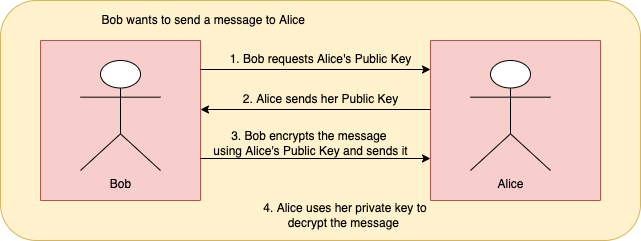
\includegraphics[width=15cm]{asym_encrp.png}
    \caption{Asymetric Encryption}
\end{figure}

\noindent A key over here is defined as a randomly generated sequence of bits. The public and private keys are closely related by 
some mathematical operations. But the question that arises here is how Bob knows that it was Alice who sent her public key. 
How can Bob authenticate the identity of Alice? This is where Digital Certificates play a crucial role, as they help in associating a public key 
with a person or an entity that allows authentication. These certificates are issued by Certification Authorities or commonly known as CAs. They are usually a third-party 
organisation (Eg: Digicert) responsible for issuing, revoking, and distributing certificates. The CA is trusted by all parties involved in 
the PKI, which would be Bob and Alice.

\noindent Now Bob can ask the CA for Alice's certificate, which contains information about Alice's public key. Since Bob trusts the CA and 
the CA is vouching for Alice, Alice's identity could be authenticated.\\
The PKI is deployed in a variety of environments over the internet to secure them, and some instances are web browsers, emails, 
file security etc~\cite{PublicKe39:online}. 

\section{Transport Layer Security}
Transport Layer Security (TLS) is a cryptographic protocol used to transfer data between applications over the internet securely. In today's day and age, 
TLS is one of the widely adopted protocols as it is majorly used in web browsers to ensure a secure session has been established. It can also be used for the safe 
transfer of data for different applications such as email, file transfers, voice-over-IP, and DNS. TLS does not secure data on the end systems but is used to 
facilitate secure data transfer from one point to another over the internet. As a result, no attacker can tamper or eavesdrop while the data is in transit. 
It is usually implemented over protocols like TCP/IP or UDP layer to secure application layer protocols like HTTP, IMAP, POP3, SMTP, and more. 
TLS was built on the Secure Socket Layer (SSL) protocol and was designed to be its replacement. It is a multilayered protocol that consists of:
\begin{itemize}
    \item \textbf{Handshake Protocol:} Authenticates the parties involved and negotiates an encryption algorithm and other parameters.
    \item \textbf{Record Protocol:} Ensures data is not tampered with when in transit using parameters negotiated during the handshake protocol.
\end{itemize}

\begin{figure}[h]
    \centering
    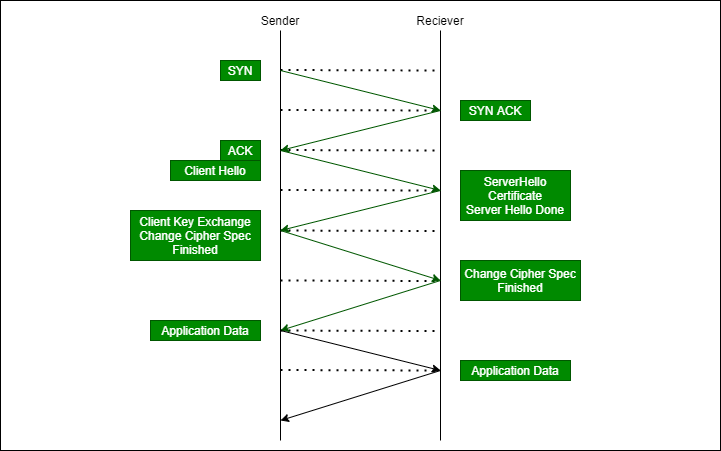
\includegraphics[width=14cm]{tls_hs.png}
    \caption{TLS Handshake Process}~\cite{Transpor60:online}
    \label{fig: TLS}
\end{figure}

\noindent Since the inception of TLS, it has been deployed in most of the web services on the internet because it protects sensitive information such as passwords, card details, emails, online chats,
browsing habits, etc. Since most websites work on a client-server model deploying TLS between the two endpoints protects sensitive information from attackers. TLS also makes use of the technique
of asymmetric cryptography which involves a key pair. In this scenario, the public key is used to encrypt the data by the sender and the receiver uses their private key to decrypt the data~\cite{rfc8446}.

\subsection{Implicit TLS v/s Opportunistic TLS}
Around the time when TLS was invented, plain text protocols like SMTP, POP3, and IMAP were already deployed heavily over the internet.
While many services supported the usage of the \textit{STARTTLS} command to upgrade the connection on the plain text ports, if a client 
did not support the same information would be transmitted in plain text before encryption was standardised. \textit{STARTTLS} or Opportunistic TLS was used 
to upgrade plain text connections to a secure one. Here the connection is upgraded after establishing the initial connection.\\
To normalise encryption over plain text protocols, new ports were decided upon by IANA. The difference here was that a TLS connection was immediately negotiated between 
the server and the client. If a server or client did not support TLS and the connection was not established, no information would be exchanged between 
the two. This is known as Implicit TLS. The use of Implicit TLS is preferred over the former to encourage consistency in 
how TLS is used~\cite{rfc8314}. The table below shows the ports used for each protocol using Implicit or Opportunistic TLS as decided upon 
by IANA~\cite{rfc6335}.
\begin{table}[h!]
    \centering
    \begin{tabular}{|c|c|c|c|c|}
        \hline
        Protocol &  Standard Port - No encryption & Implicit TLS Port & Opportunistic TLS Port\\
        \hline
        SMTP  &   25    &   587 &   25\\ 
        \hline
        POP3  &   110   &   995 &   110\\
        \hline
        IMAP &   143    &   993 &   143\\  
        \hline
        HTTP    &   80  &   443 &   -\\
        \hline
    \end{tabular}
    \caption{Implicit TLS vs Opportunistic TLS Ports}
    \label{tab:TLSports}
\end{table}

\subsection{TLS Certificates}
TLS certificates verify the ownership of a public key and are essential to secure connections and transactions over the internet. 
They are usually issued by some Certification Authority (CA) by signing the certificates indicating that the CA has verified the ownership. 
Whenever a user tries to connect to a server, the server sends them a certificate, and then the user verifies the server's certificate using the CA certificate 
present on the user's machine to establish a TLS connection. The certificates usually contain the following fields of information~\cite{rfc5280}:
\begin{itemize}
    \item Subject Domain Name
    \item Subject Organisation
    \item Issuing CA
    \item Alternative Subject Name 
    \item Date of Issue 
    \item Expiry Date 
    \item Public Key 
    \item Digital Signature by the issuing CA
\end{itemize}

\subsection{TLS Cipher Suites}
A cipher suite is defined as a set of cryptographic algorithms that are used by TLS to encrypt the information. It provides crucial 
information about securing data when using different network protocols like SMTP, HTTPS, POP3, etc. A cipher will dictate what algorithm is 
best suitable to make a secure and reliable connection to the server. A cipher suits provides the following information to a server:
\begin{itemize}
    \item \textbf{Key Exchange Algorithm:} Data over the internet is encrypted using a key. This provides the client and server with which algorithm to use for encryption/decryption of data.
    \item \textbf{Authentication Algorithm:} The server needs to verify the client's identity before sending or receiving any data. This field specifies that algorithm.
    \item \textbf{Bulk Data Encryption:} This is to ensure the secure transfer of data. 
    \item \textbf{Message Authentication Code Algorithm:} A MAC algorithm is sent along the with data to verify the contents of the data. 
\end{itemize}

\begin{figure}[h!]
    \centering
    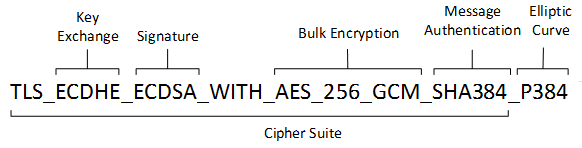
\includegraphics[width=10cm]{tls-cipher-suite.png}
    \caption{TLS Cipher Suite}~\cite{CipherSu69:online}
    \label{fig: CipherSuites}
\end{figure}

\subsection{Fingerprint SHA-256}
The concept of a key pair was introduced above. A fingerprint is defined as a short sequence of bytes used to identify a longer public key and is generated
by applying a hash function on a public key. SHA stands for Secure Hash Algorithm, which is used to shorten data into a minor sequence. The resulting 
output cannot be cracked unless a brute force attack is used, and this is where hashing differs from encryption. SHA256 is a popular cryptographic
algorithm that, if applied to a number consisting ``n'' bits, will return a 256-bit value. It is widely used in digital certificates and signatures. 

\section{Application Layer Protocols}
This section describes the ports we scan and the protocols associated with the ports. 
\begin{table}[h!]
    \centering
    \begin{tabular}{|c|c|c|}
        \hline
        Port &  Protocol\\
        \hline
        22  &   SSH\\ 
        \hline
        25  &   SMTP\\
        \hline
        110 &   POP3\\  
        \hline
        143 &   IMAP\\  
        \hline
        443 &   HTTPS\\ 
        \hline
        587 &   SMTP Submit\\  
        \hline
        993 &   IMAPS\\ 
        \hline
    \end{tabular}
    \caption{Ports Scanned}
    \label{table:alports}
\end{table}

\subsection{Secure Shell Protocol}
The Secure Shell (SSH) is a network communications protocol that enables two computers to communicate and share data remotely. 
Communication between the two machines is encrypted, meaning this protocol can be used over an insecure network to make it secure.
SSH consists of three layers: 
\begin{itemize}
    \item \textbf{Transport Layer:} Establishes safe connections between the server and the client for communications after the authentication process has been validated. Oversees data encryption, decryption, and integrity and provides caching and compression if needed. 
    \item \textbf{Authentication layer:} Conducts the authentication process, i.e.\ verifies the identity of the user.
    \item \textbf{Connection Layer:} Manages the communication between the two machines once authentication is completed and handles the opening and closing of each session. 
\end{itemize}

\noindent SSH requires a login from the user to start performing operations on the remote machine and can be used for the safe transfer of data. 
It works on a client-server model, i.e.\ the client will initiate the process by pinging the server, and in turn, the server responds to the client prompting them 
to finish the authentication process. The SSH server listens on some TCP/IP ports designated for SSH, and usually, TCP/IP port 22 is reserved for SSH servers.
Clients contact the server on this port to start the connection process~\cite{rfc4254}.

\begin{figure}[h!]
    \centering
    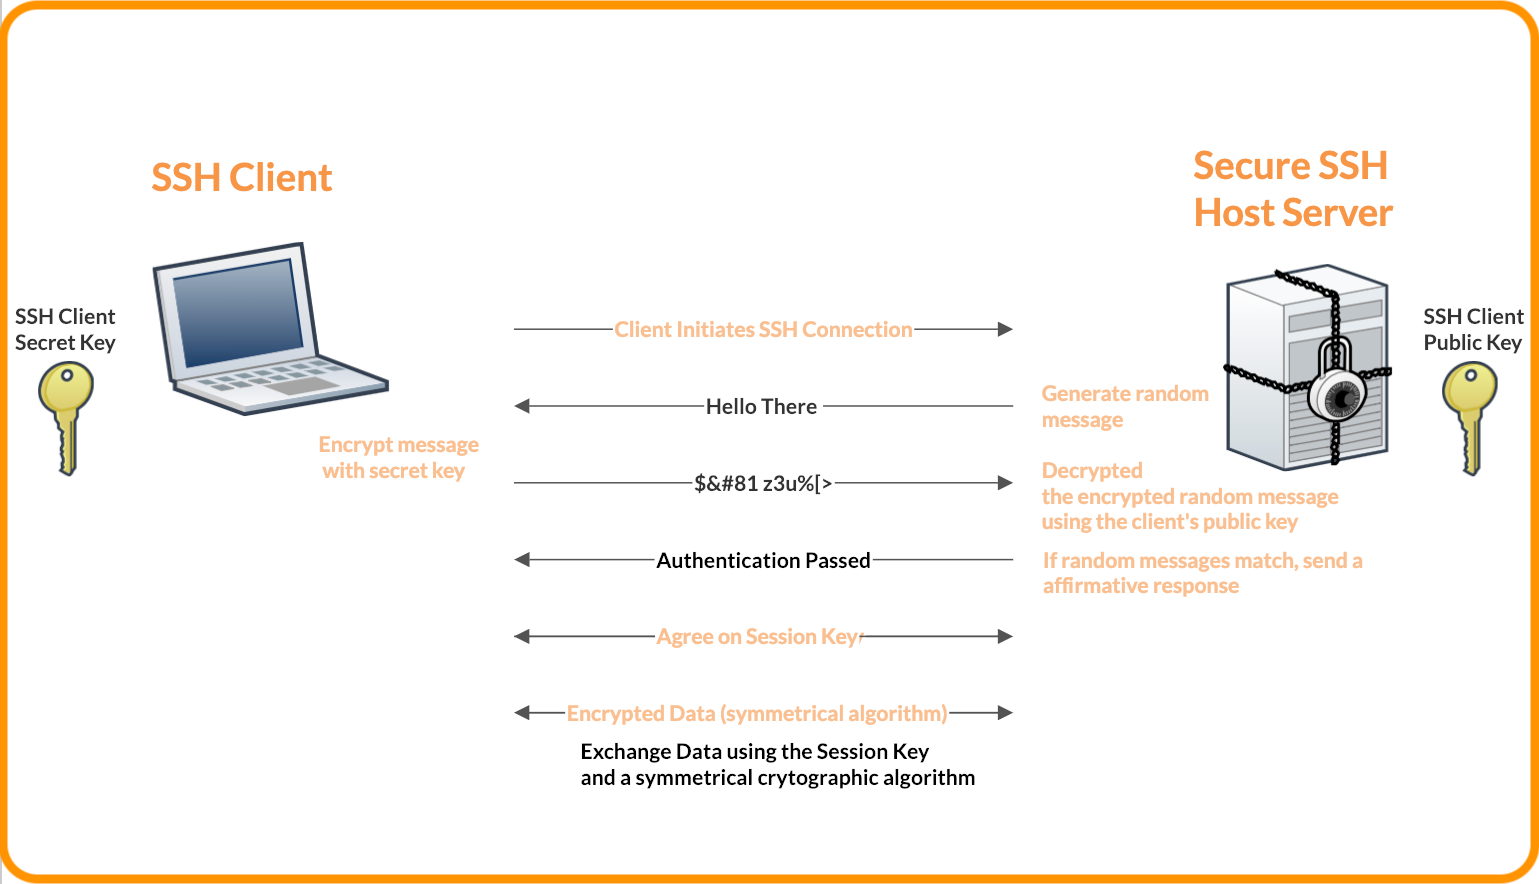
\includegraphics[width=13cm]{ssh_working.png}
    \caption{SSH Process}~\cite{LearnSSH25:online}
    \label{fig: SSHworking}
\end{figure}

\noindent SSH uses asymmetric cryptography similar to the PKI for the authentication process between the client and the server and uses symmetric encryption and other hashing algorithms
to encrypt the data transfer between the client and the server, ensuring privacy and integrity. Each SSH server should have at least one host key to ensure 
that the client communicates with the correct server during the key exchange. Ideally, each host should have a unique key, as key sharing between hosts can leave the host 
susceptible to man-in-the-middle attacks. However, key sharing may be acceptable and even practical (for instance, multiple hosts sharing keys but all under one entity). The Secure Shell Protocol is widely adopted and used for various purposes by individuals and Corporations. 
Some use cases are remote access to machines, port forwarding, virtual private networks, and many more.  

\subsection{SMTP/ (S)}
Simple Mail Transfer Protocol is used to transfer mail reliably and efficiently. A two-way connection is established with an SMTP server when an SMTP client wants to transmit a message. The main objective of this protocol is to transfer mail messages to an SMTP server 
or to report failure to incase it fails to do so. Traditional SMTP operates over assigned port 25 and usually does not provide encryption, meaning that the client and server communicate over the internet in plain text~\cite{rfc5321}. This can be considered a significant flaw as 
all communications are susceptible to eavesdropping or man-in-the-middle attacks while emails are in transit. 
SMTP over TLS or SMTPS was introduced to encrypt these communications. By using SMTP over TLS, one is wrapping SMTP commands inside 
a TLS connection. Usually, port 587 is used for SMTPS compared to port 25 for SMTP to distinguish between the two.

\noindent With the use of SMTP over TLS, the client waits for the \textit{STARTTLS} keyword from the SMTP server. After that, the TLS handshake 
protocol is completed. After the handshake is completed, the client and the server decide whether to continue ahead with the session based 
on the current privacy achieved. Some client-servers might choose to continue ahead even if no TLS authentication was attained, as traditionally 
SMTP operates without any encryption, while others may only decide to continue with the session based on specific authentication and 
privacy achieved..~\cite{rfc2487}.

\subsection{POP3 / (S)}
Post Office Protocol Version 3 or POP3 is a standard mail protocol used by mail servers and their clients to receive emails from a remote 
server and send it to a local client. It is a client-server protocol in which email is received and stored on a mail server, and a recipient of an email client 
can download emails from that server which enables the client to view the email offline. POP3 is embedded into most email clients. Once the 
email is on the client, POP3 can be configured to delete the email from the server or save the email for a specific period, allowing 
clients to download the mail as many times. The standard port assigned to POP3 is port 110, but usually, communication is over 
plain text on this port, but a secure connection can be established using the \textit{STARTTLS} command on this port. In case the client wants to 
connect securely, POP3 over TLS is used that is assigned to port 995~\cite{rfc1939}.

\subsection{IMAP/ (S)}
The Internet Message Protocol or IMAP is a standard mail retrieval protocol used to download mail messages by email clients. It enables 
users with control over mail boxes and enables with to organise them as per requirements. The port assigned to the IMAP protocol is 143, 
but it does not support encryption over that port. To secure it the \textit{``STARTTLS''} command can be used. Alternatively, port 993 can be used 
that supports IMAP or TLS (IMAPS) that establishes a TLS connection immediately.~\cite{rfc9051}.

\subsection{HTTPS}
HTTPS or HTTP over TLS is an alternative to simple HTTP over TCP. The difference here is that the HTTP client should also act as a TLS 
client. The client should initiate the connection, but before making an HTTP request, it should establish a TLS session by initiating the 
TLS handshake protocol. Once the handshake is completed, the client can start making HTTP requests to the server. All data exchanged between 
the client and the server is sent as TLS application data. To distinguish between HTTP over TCP and HTTP over TLS, both protocols have been 
assigned different port numbers. HTTP operates over port 80 while HTTPS operates over port 443~\cite{rfc2818}.

\section{Technology Evolution}
The development of the surveying program was previously done in 2017/18 using Python2. However, Python3 has gained popularity and has been 
widely adopted by corporations, individuals, and others. There are few notable differences between the two, and specific Python3 versions 
provide better performance than Python2 versions. Since January 1, 2020, support for Python2 has been discontinued. That means there
will be no further improvements for Python2 even if a significant bug or security flaw is found~\cite{10.5555/1593511}. Popular libraries 
like Pandas, NumPy, and many more have officially stopped supporting Python2 versions, which makes it even more critical to migrate the current code to 
Python3~\cite{Installa51:online}.\\
The previous program used ZGrab1 to run the scans back in 2017/18, and since then, ZGrab2 has been released, which has depreciated the last version. 
It contains a revamped framework that has simplified the tools' usage and allows individuals to add custom protocols over various ports by building them on their own using Golang. It has 
integration tests available which can help the development process and can be efficiently run using Docker~\cite{merkel2014docker,zgrab2Github}.\\
There were also some minor changes to how Maxmind ships the data needed for the program to work. Additional scripts and modifications to current ones were carried out to get 
the countrywide IP data to carry out the scans.

\newpage
\section{Code Refactoring}
\label{refactortechs}
Code refactoring can be defined as the restructuring of code to improve code readability, reduce complexity, and improve the 
maintainability and efficiency of the program. The refactoring process should contribute to the above factors, 
but the program's functionality should not be compromised. Refactoring enables developers to gain an in-depth understanding of 
the program and enables them to expand the program quickly by integrating more features efficiently and reducing the amount 
of technical debt.

\noindent Technical debt, also known as code debt, refers to when development is rushed or when code delivery is prioritised over 
writing quality code. To ensure code refactoring has yielded benefits, one needs to define a few metrics like \textit{``\% of duplicate code''} \cite{ThePower10:online}. 
Techniques like unit testing and functionality tests need to be performed regularly in order to ensure the refactoring process is beneficial~\cite{TheCompl71:online}. 
Refactoring a program should be started by analysing the current code and checking whether refactoring is required. 
There are a few standard practices defined in the software engineering community to carry out the process of code refactoring. 
Some of the practices used in the project include:
\begin{itemize}
    \item \textbf{Inline:} Simplifying code by eliminating unnecessary elements. 
    \item \textbf{Extract:} Break down code into smaller fragments and then move these fragments into a different method. 
    \item \textbf{Abstraction:} Reduce the amount of duplicate code by identifying points of similarity. \cite{refactoring}  
\end{itemize}

\chapter{Related Work}
%%litreview
\label{relevantlit}
Henniger et al.~\cite{180213} perform Internet-wide scans of the entire IPv4 address space for hosts that listen on port 22 (SSH) or 
port 443 (HTTPS) using the NMap tool. NMap is an open-source network scanner that is used for network audits. They perform TLS or SSH handshakes
on hosts that listen on port 443 or port 22, respectively, and gather most of the data that might help discover weak keys. 
For TLS, they capture most of the metadata like certificate information and other X.509 certificate fields. For SSH, they collect the host keys 
using a simple client developed in C. All of the scans and data processing were carried out using Amazon's EC2 service, which provided them with 
an infrastructure to collect and analyse data efficiently. After processing the information, they identify some patterns between 
a host that shares keys and try to pinpoint some of the causes behind these. 
In the TLS protocol, the server sends its public key in a TLS certificate during the handshake stage. This key is 
used to provide a signature during the handshake stage or can be used to encrypt session details depending on whether RSA or DSA encryption algorithm is 
negotiated between the client and the server. Similarly, in the SSH protocol, the host key allows the server to authenticate itself to the client by providing a signature during 
the handshake stage. In both these protocols, if the private keys are known by an attacker and depending on the type of the 
encryption scheme (RSA or DSA), an attacker can perform different attacks like man-in-the-middle or decrypt the message containing
the session key and, in turn, use that to decrypt the entire session.\\
\cite{180213} further computes the private keys using the weak public keys by exploiting the weakness of RSA and DSA algorithms when used 
with insufficient randomness. As a result, they can compute private keys for 0.50\% of the total TLS hosts and 1.06\% of the SSH hosts found from their 
respective public keys since the key pair is related mathematically.  
They scanned 12.8 million TLS hosts and only obtained 5.8 million unique certificates for them. For SSH, they scanned 10.2 million hosts 
and obtained 6.2 million unique keys. Indicating that about 61\%  and 65\% of the TLS and SSH hosts shared the same key as another host 
in the scans. Investigating the causes of this key sharing between hosts, they found that some of the key sharing was not 
due to vulnerabilities in the infrastructure but large hosting providers that used a single key for multiple IP addresses. Another significant 
reason was TLS certificates that belonged to the same organisation. Therefore, they excluded exceptions from their data analysis process and clustered the 
remaining host that shared keys.\\\\
Dr.~Farrell's work on surveying long-term cryptographic keys for SSH, mail, and web protocols is relevant literature as this project builds 
directly from~\cite{cryptoeprint:2018:299}. The research surveys keys for ten countries and describes scans that involved hosts 
in Ireland and Estonia. The program~\cite{sftcdsur24:online} used to carry out these scans made use of Censys databases in 2017 and Maxmind databases in 2018 
to perform these scans. Then ZMap and ZGrab are used to collect data on hosts that listen on port 25, and further, the data is processed and analysed.
From one of the scans in Ireland carried out in 2018 that involved 18,268 hosts that offer at least one SSH or TLS service, approximately 
53\% hosts shared keys. Out of the 54,447 host-port combinations, only 36\% unique keys were seen through that scan. The research also reports 
key sharing among countries and shows how widespread this resue is. The clustering of hosts is based on the fingerprint information collected from 
SSH hosts and hosts that use TLS on top of the standard protocols. ``If any two IPs share a fingerprint irrespective of the port, they are clustered 
together'' to check for key reuse among hosts. Other metadata during TLS and SSH handshakes are collected for extensive data analysis. 
After the data analysis, some scripts are used to visualise the cluster information to communicate with local asset holders to understand better the causes 
of this key reuse from an asset holder's point of view and how the network security infrastructure can be improved. 
\cite{cryptoeprint:2018:299} introduces a metric called HARK \%: ``Host that is resuing keys'' for quantifying this key reuse. One of the main 
hypotheses of the work was to see if there is a correlation between the HARK\% and improvement in the security posture.

\noindent As outlined in section~\ref*{resobjectives}, one of the goals of this project is to migrate the code to Python3, refactor it to increase readability, and 
carry out some optimisation to reduce the memory overhead. This is critical since most of the work carried out in~\cite{cryptoeprint:2018:299} was done using a combination of Python2 and Bash Scripts, is quite memory intensive, 
and Python2 has deprecated since. The project also checks how key reuse has evolved over the years since 2018. 

\section{Summary}
Summarising the section above, there is widespread key reuse in a vulnerable due to a variety of reasons. 
Although a single entity cannot be blamed, regular scanning might help in better understanding some of the causes and dangers behind the 
key reuse from both an asset holder and a user point of view. 
\noindent This section summaries some of the causes and dangers of this key reuse as described in~\cite{180213,cryptoeprint:2018:299}.   
\subsection{Causes of Key Reuse}
\begin{itemize}
    \item \textbf{Hardcoded Keys:} Many devices are shipped with default keys by manufacturers in the firmware of the device. This contributes
    to key reuse as some users might not have the knowledge on how to change these keys.
    \item \textbf{Lack of Randomness:} A significant reason for key reuse was the lack of entropy during key generation. 
    This might be due to faulty random number generators or due to high costs of computations. 
    \item \textbf{Multihomed Hosts:} If a host has more than one network interface with different IPv4 addresses, it will show as individual 
    hosts in the scans. 
    \item \textbf{Virtual Machines:} If a few hosts share a key and all of those hosts are VMs, that will contribute to this. However, 
    in this case, it can be passed as acceptable as all hosts are under one physical entity.
\end{itemize}
\subsection{Dangers of Key Reuse}
\begin{itemize}
    \item \textbf{Cross Protocol Attacks:} Even though new versions of TLS are available, the migration from the older version is still slow. 
    Key reuse can increase the probability of cross-protocol attacks, and old versions of TLS/SSL may be vulnerable to these. 
    \item \textbf{Masquerading:} If asymmetric encryption is used for authentication, then key reuse may enable an attacker to pose as a host if 
    a breach of a host occurs in a cluster. 
    \item \textbf{Credential Exposure:} If sensitive information like passwords are sent using plain text protocols like SMTP, and if an 
    active attacker can masquerade as a host in a cluster, they can capture those credentials. 
    \item \textbf{Cost of Leaks:} Since private keys are usually stored locally, there is always some probability of leaks due to hardware failures. 
    If there is a leak from a host that shares keys with other hosts, this will affect all of them. Moreover, as the cluster size increases, the impact 
    of these leaks would also increase. 
\end{itemize}
\chapter{Implementation}
%%implemenation 
This chapter specifies the approach taken to execute the project. Section~\ref*{codeoverview} gives an overview and 
describes the technologies used to carry out this project. Sections~\ref*{envsetup},~\ref*{stage1},~\ref*{stage2},~\ref*{stage3} 
explain how the program operates, and~\ref*{additions} provides information about some additional tooling developed to get better insight into the data. 
Section~\ref*{refactoring} provides an insight into the techniques used to refactor and optimise the orignal code~\cite{sftcdsur24:online}. 
The last section talks about the challenges faced during implementation.  

\section{Overview}
\label{codeoverview}
The program for surveying keys~\cite{sethr07s72:online} had various stages in which it performed different functions. Figure~\ref*{programstruct} depicts the flow of the program, and it can be divided into the following stages:
\begin{itemize}
    \item \textbf{Environment Setup:} Downloads all the required dependencies required for the program to work, including Python libraries, Maxmind databases, ZMap, ZGrab, and setups Golang.
    \item \textbf{Stage 1:} This stage can be called the Maxmind stage, where the MaxMind APIs are set up and filters out IP addresses for the country selected. 
    \item \textbf{Stage 2:} This is the scanning stage where ZMap and ZGrab are used. The IPs from Stage 1 are scanned using ZMap for open port 25. Once those IPs are available, ZGrab is used to capture data for the ports. 
    \item \textbf{Stage 3:} The final stage of the program where data from Stage 2 is processed, stored and analysis are carried out. 
\end{itemize}
\begin{figure}[h]
    \centering
    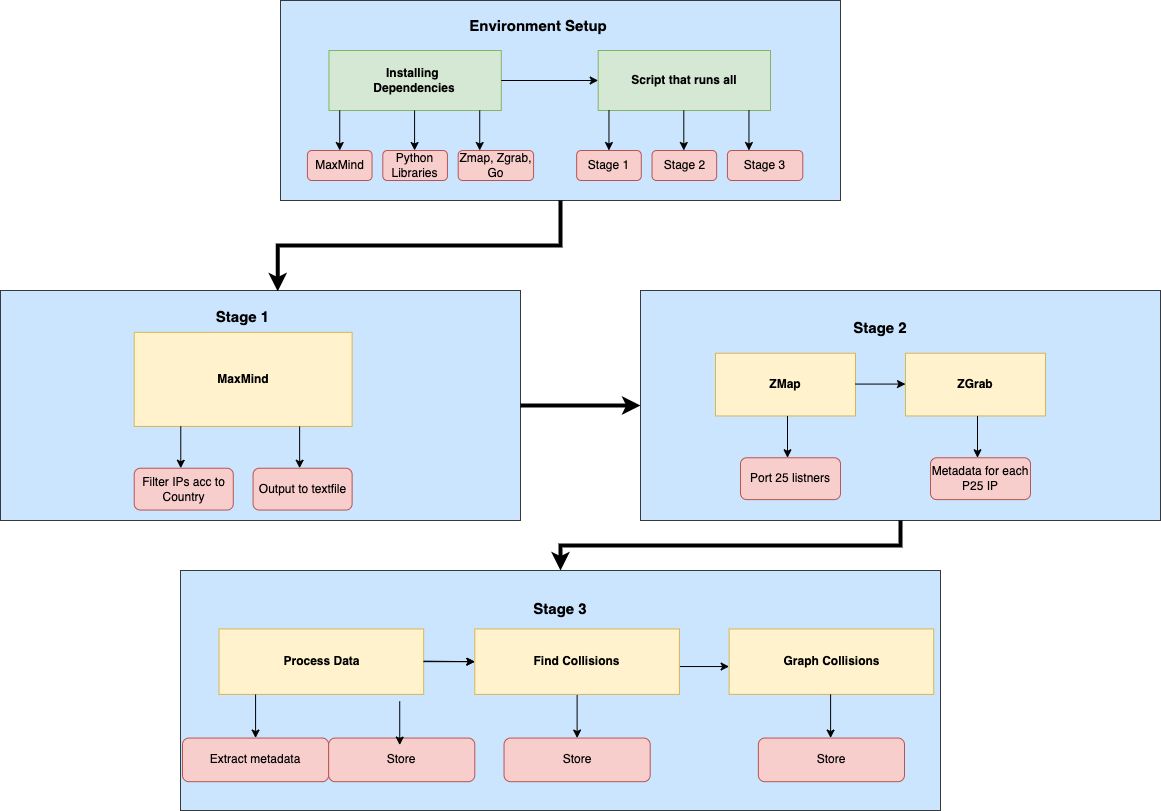
\includegraphics[width=18cm]{programstruct.drawio.png}
    \caption{Program Strcuture}
    \label{fig: Program Strcuture}
    \label{programstruct}
\end{figure}

\subsection{Technologies Used}
The following lists the technologies that were used to carry out the project:
\begin{itemize}
    \item \textbf{Python3:} Majority of the program was developed using Python3. Used for data processing, visualisation, and calling APIs and tools used.
    \item \textbf{Bash Script:} Used for automation of tasks, downloads and specific data extraction tasks.
    \item \textbf{ZMap:} Port scanner used to identity open port 25 listeners. 
    \item \textbf{ZGrab:} Banner Grabber to obtain information about hosts in question.
    \item \textbf{Maxmind:} Used databases and APIs provided by MaxMind to carry out the network scans.
    \item \textbf{Pylint:} A code analysis tool used to measure code quality and enforce a standard coding structure. 
    \item \textbf{cProfile and pstats:} A deterministic profiling tool used to optimise memory consumption and runtime.
\end{itemize}

\section{Environment Setup}
\label{envsetup}
Before the program execution begins, a script called \textit{``install-deps.sh''} downloads and installs all dependencies for the program to work. It starts by creating directories where the source code 
is available and another directory where the results for each scan are stored. After doing so, it will install dependencies like the Python libraries required, ZMap, ZGrab, and the MaxMind databases. 
It also installs Golang and configures the \textit{``gopath''} as ZGrab requires a valid \textit{``gopath''} to function. Since this program was the last run in 2018, the Maxmind databases have changed significantly. Therefore, 
an additional script called \textit{``MMIPs.py''} was developed to create a CSV dataset called \textit{``GeoIPCountryWhois''} was required for the program to run. The Python script takes in two CSV files as input that 
contain the entire IPv4 network blocks with their associated Geonames. In addition, there was another CSV file that had the Geonames and the country code and name associated. The script 
processes these two CSV files and then maps the IPv4 network blocks to their associated country code (and country names) using the Geonames. Finally, it produces the final CSV dataset needed.

\section{Stage 1: Maxmind Stage}
\label{stage1}
The program's first stage was to filter out the IP addresses for the country specificed to scan. For this project, the country choof interest was Ireland. 
The top script \textit{``skey-all.sh''} does all the work and calls these stages sequentially, as indicated in figure~\ref*{programstruct}. The script \textit{``IPsFromMM.py''} performs the first stage. 
It takes in the input file \textit{``GeoIPCountryWhois.csv''} and filters the IPv4 CIDRs according to the selected country. The final output from 
this stage is a text file that contains IPv4 CIDRs for the country chosen.

\section{Stage 2: Port Scan and Banner Grab}
\label{stage2}
This stage involved two parts. The first one was using ZMap to check for open port 25 listeners, and the next was using ZGrab on those hosts 
to gather the SSH and TLS meta-data.

\subsection{ZMap}
After getting the list of IPs for the country selected, the program moves onto the second stage and uses ZMap to map which IPs listen on port 25. ZMap is called 
using the main script \textit{``skey-all.sh''} as it requires system privileges. The final output from ZMap is a list of IP addresses that listen on port 25. 
Figure~\ref*{fig:zmapout} shows how the ZMap output looks like. It expands each IP in CIDR notation to the IP range and pings each IP in 
the range using the TCP SYN scan. The fields indicate the time left on the scan, the ``send: 2947'' shows that ZMap has pinged 2947 IPs address, 
and the ``recv:2'' means that ZMap has found two port 25 listeners. The ``hitrate: 0.07\%'' indicates that out of the total IPs pinged 0.07\%  
were port 25 listeners.  
\begin{figure}[h]
    \centering
    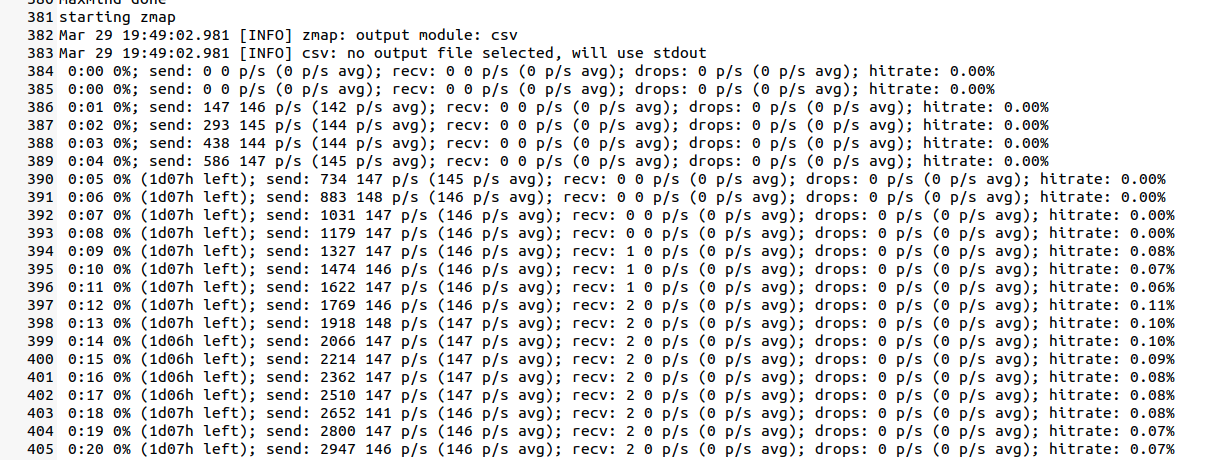
\includegraphics[width=18cm]{zmap_output.png}
    \caption{ZMap Output}
    \label{fig:zmapout}
\end{figure} 

\subsection{ZGrab}
The following process in this stage was to gather metadata about each port for IP addresses we obtained from ZMap. This is where the ZGrab2 tool was used, and the process was done using the script 
\textit{``FreshGrab.py''}. The script specifies the ZGrab parameters and calls the ZGrab binary. It requires an input file that is a list of IPs (ZMap output) and first verifies whether the IP belongs to the 
specified country using methods defined that make use of the Maxmind databases and APIs. If the IP does not match the country according to Maxmind, they are marked as ``out of country'' and are not processed further. 
The remaining IP addresses are processed using the ZGrab tool. Since the output is in JSON, the data is stored in a file called \textit{``records.fresh''} that 
contains one JSON structure per line. Each line has information about all seven ports for each IP. This part of Stage 2 can take anywhere 
from a few hours to a day to complete since the scan rate of the ZGrab tool was limited by adding a 100 ms wait between each IP so as not to cause any congestion in the network. 
\pagebreak

\begin{lstlisting}[caption={ZGrab2 Parameters}, captionpos=b, label={zgrabparams}]
    ports=['22', '25', '110', '143', '443', '587', '993']
    ztimeout=' -t 2'
    pparms={ 
        '22': 'ssh -p 22',
        '25': 'smtp -p 25 --starttls',
        '110': 'pop3 -p 110 --starttls',
        '143': 'imap -p 143 --starttls',
        '443': 'http -p 443 --use-https',
        '587': 'smtp -p 587 --smtps',
        '993': 'imap -p 993 --imaps',
        }
    for port in ports:
        cmd=zgrab_path + " " +  pparms[port] + ztimeout
        proc=subprocess.Popen(cmd.split(),stdin=subprocess.PIPE,stdout=subprocess.PIPE)
        pc=proc.communicate(input=ip.encode())
\end{lstlisting}

\noindent Listing~\ref*{zgrabparams} shows how ZGrab is used in the \textit{``FreshGrab.py''} script. The parameters specify the protocols and 
associated ports for it to scan for. To capture the TLS metadata for the plain text ports, the \textit{STARTTLS} command was used,
and implicit TLS for the other ports.

\section{Stage 3: Data Processing and Visualisation}
\label{stage3}
Stage 3 of the program involved parsing out the metadata from the JSON structures the project required, performing DNS and reverse DNS lookups, 
storing the data, and finding where the same key is being used for each IP for every possible host-port combination. Stage 3 can be broken down as follows:

\subsection{Data Processing}
The script that handles the data processing is \textit{``SameKeys.py''} and starts by iterating through data for each IP address in file \textit{``records.fresh''}. 
Since plenty of metadata is captured for each IP, the data is stored using Python, a class instance with multiple attributes. 
Then, the program starts by performing reverse DNS lookups for the IP and storing the names obtained in the same class instance. 
After that, Fully Qualified Domain Names, TLS certificates, and fingerprint information are parsed and stored for every port. 
The FQDNs are stored to assist with verifying the asset owners that are operating the said service. The program also keeps 
the information about the autonomous system associated with each host using the Maxmind databases. The methods to parse and store these 
fields are defined in the \textit{``SurveyFuncs.py''} script. Before moving onto the analysis stage, the program verifies names associated with the 
IPs by performing DNS lookups with the SANs related to the IP. The program only stored a maximum of 20 SANS per host, as some hosts have a large amount of SANs that 
slow down the program. If the IP addresses from the DNS lookup match the IP in \textit{``records.fresh''}, it is 
recorded as ``good''. Otherwise, it is recorded as ``bad''. The IPs marked as ``good'' with a key are stored in a JSON file for further analysis. 
The same is done with the ``bad'' IPs, and another file contains both IPs marked as both ``good'' and ``bad'' with their associated information. 
Appendix A provides the output of ZGrab and shows the information collected for all seven ports for each IP address. 
The appendix only provides data for one IP address in JSON format. 

\subsection{Data Analysis}
The data analysis process entails checking for the duplicate keys for different services within and across IPs. The clustering is based on fingerprint SHA-256 for each service. 
If a specific key is shared by two hosts irrespective of the protocol, they are put in the same cluster. This is because it is not uncommon to see key reuse for different services, as proved in~\cite{cryptoeprint:2018:299}. 
When key reuse is identified, the initial collisions are cross-checked with each other and are merged if the same key is being used there. 
Once, this is complete three files are produced as follows: 
\begin{itemize}
    \item ``collisions.json'': Contains key reuse information among hosts.
    \item ``dogies.json'': Contains information about IP that are recorded as ``bad''.
    \item  ``all-key-fingerprints.json'': Contains information that is included in the first two files. 
\end{itemize}

\subsection{Data Visualisation}
After obtaining the data as describe abovethe collisions are graphed using the Graphviz library in Python. The file used to graph the 
collisions is \textit{``collisons.json''}. Each host in the file is iterated through, and the hosts with the same cluster number are finally graphed using custom 
methods defined based on Graphviz.\\\\
\pagebreak
\begin{figure}[h!]
    \centering
    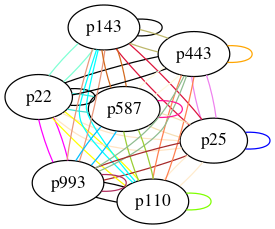
\includegraphics[width=11cm]{legend.png}
    \caption{Graph Legend}
    \label{fig:graphsleg}
\end{figure}

\noindent Figure~\ref*{fig:graphsleg} represents the graph legend, and the graphs can be visualised as follows:

\begin{itemize}
    \item The nodes are represented as IP addresses.
    \item The colour of the nodes represents the entities or hosts.
    \item The edges represent key reuse across ports. 
    \item The colour represents the pair port combination. 
\end{itemize}  

\section{Additional Tools}
\label{additions}
Some additional scripts are available that provide in-depth analysis of the data collected. For example, the script \textit{``ProtocolVersions.py''} 
provides an insight into the TLS/SSL versions seen throughout the scans and provides a count for them. It also provides details of 
the SSH versions seen on port 22. More tooling offers information on how many IP addresses were mapped by ZMap, how many host port 
combinations are there, how many unique fingerprints are seen, and many more. All of these scripts were used that assisted in the analysis of the results.

\section{Code Migration, Refactoring and Optimisation}
\label{refactoring}
One of the primary goals of this project was to migrate the code to Python3 and refactor it to increase readability, improve the structure, 
and optimise the run time and memory usage. This section gives details about the migration and the refactoring process. It also provides 
information about the techniques used to increase code performance.

\subsection{Code Refactoring}
The refactoring process was carried out by first analysing the entire program to check for duplicate code. Methods that were complex methods and involved heavy 
nesting were identified. In the \textit{``SameKeys.py''} script where the data processing takes place, all information parsing was done manually according 
to the JSON headers fields for each port. Due to this, the code was not so readable and looked complex. Therefore, the techniques 
outlined in section~\ref*{refactortechs} were used to carry out the refactoring. The following code snippets give an example of this. 

\begin{lstlisting}[caption={Code before Refactoring}, captionpos=b, label={codebefore}]
    try:
        p25=j_content['p25']
            if thisone.writer=="FreshGrab.py":
                banner=p25['data']['banner'] 
            else:
                banner=p25['smtp']['starttls']['banner'] 
            ts=banner.split()
            if ts[0]=="220":
                banner_fqdn=ts[1]
                nameset['banner']=banner_fqdn
            elif ts[0].startswith("220-"):
                banner_fqdn=ts[0][4:]
                nameset['banner']=banner_fqdn
    except Exception as e: 
        print >> sys.stderr, "FQDN banner exception " + str(e) + " for record:" + str(overallcount) + " ip:" + thisone.ip
        nameset['banner']=''
    try:
        if thisone.writer=="FreshGrab.py":
            tls=j_content['p25']['data']['tls']
            cert=tls['server_certificates']['certificate']
        else:
            tls=j_content['p25']['smtp']['starttls']['tls']
            cert=tls['certificate']
            fp=cert['parsed']['subject_key_info']['fingerprint_sha256'] 
            get_tls(thisone.writer,'p25',tls,j_content['ip'],thisone.analysis['p25'],scandate)
            get_certnames('p25',cert,nameset)
            thisone.fprints['p25']=fp
            somekey=True
    except Exception as e: 
        print >> sys.stderr, "p25 exception for:" + thisone.ip + ":" + str(e)
        pass   
\end{lstlisting}
\begin{lstlisting}[caption={Code After Refactoring}, captionpos=b, label={codeafter}]
    try:
        p25 = j_content['p25']
        bn = "y"
        if thisone.writer == "FreshGrab.py":
            banner_fqdn = get_mail_data(p25, bn)
        else:
            banner = p25['smtp']['starttls']['banner']
            nameset['banner'] = banner_fqdn
    except Exception as e:
        print(sys.stderr, "FQDN banner exception " + str(e) + " for record:" + str(overallcount) + " ip:" + thisone.ip)
        nameset['banner'] = ''
    try:
        if thisone.writer == "FreshGrab.py":
            data = j_content['p25']['data']['smtp']['result']['tls']
            cert, fp = get_mail_data(data, None)
        else:
            tls = j_content['p25']['smtp']['starttls']['tls']
            cert = tls['certificate']
        get_tls(thisone.writer, 'p25', data, j_content['ip'], thisone.analysis['p25'], scandate)
        get_certnames('p25', cert, nameset)
        thisone.fprints['p25'] = fp
        somekey = True
    except Exception as e:
        print (sys.stderr, "p25 exception for:" + thisone.ip + ":" + str(e))
        pass
\end{lstlisting}
Listing~\ref*{codebefore} and Listing~\ref*{codeafter} shows the code before and after refactoring respectively. In this instance, a method 
was introduced called \verb|get_mail_data(data,banner)| that was used to extract the banner information for port 25, but also to gather 
the TLS certificate and fingerprint data for all mail protocols instead of doing this manually for each mail port.\\
Other methods were created as well, and the existing ones were modified for simplicity. This was done to decrease the number of 
lines of code in the \textit{``SameKeys.py''} script and to avoid writing duplicate code. It also had another benefit that in case there 
are changes to the ZGrab output in the future, one will have to make changes in the program at one point instead of doing it manually 
for all ports.\\\\
Another instance where refactoring was carried out was in the \textit{``SurveyFuncs.py''} script that contains custom utility functions. 
While it is still somewhat acceptable to have manual code in this script as it is not used directly, refactoring was carried out here 
to improve performance. For example, existing methods that were used to call the Maxmind APIs contained a lot of nesting of \textit{if} 
statements and \textit{for} loops. To decrease the nesting, the abstraction technique was used to break down the nested statements by defining 
different methods to perform the same function overall. 

\subsection{Code Optimisation}
To optimise this program, memory analysis had to be carried out that gave information about the memory overheads of the program and identified what was 
taking the most amount of time to complete the whole process. This analysis was carried out using the \textit{cProfile} and \textit{pstats} 
libraries available in open-source. A profile here is defined as a ``set of statistics that describes how often and for how long various parts 
of the program are being executed''~\cite{ThePytho56:online}. When used with the scripts, this library gives a detailed report about how the program behaves. 
It gives information about the number of monitored calls and how many of those were primitive or recursive. In addition, it provides the total time spent 
in each method and the cumulative time spent in the method and all sub-methods. Once this data was available, it was investigated, and areas of the program were 
identified where bottlenecks were being created. Finally, alternative solutions were explored to decrease run time and to decrease memory usage.
\newpage

\begin{figure}[h!]
    \centering
    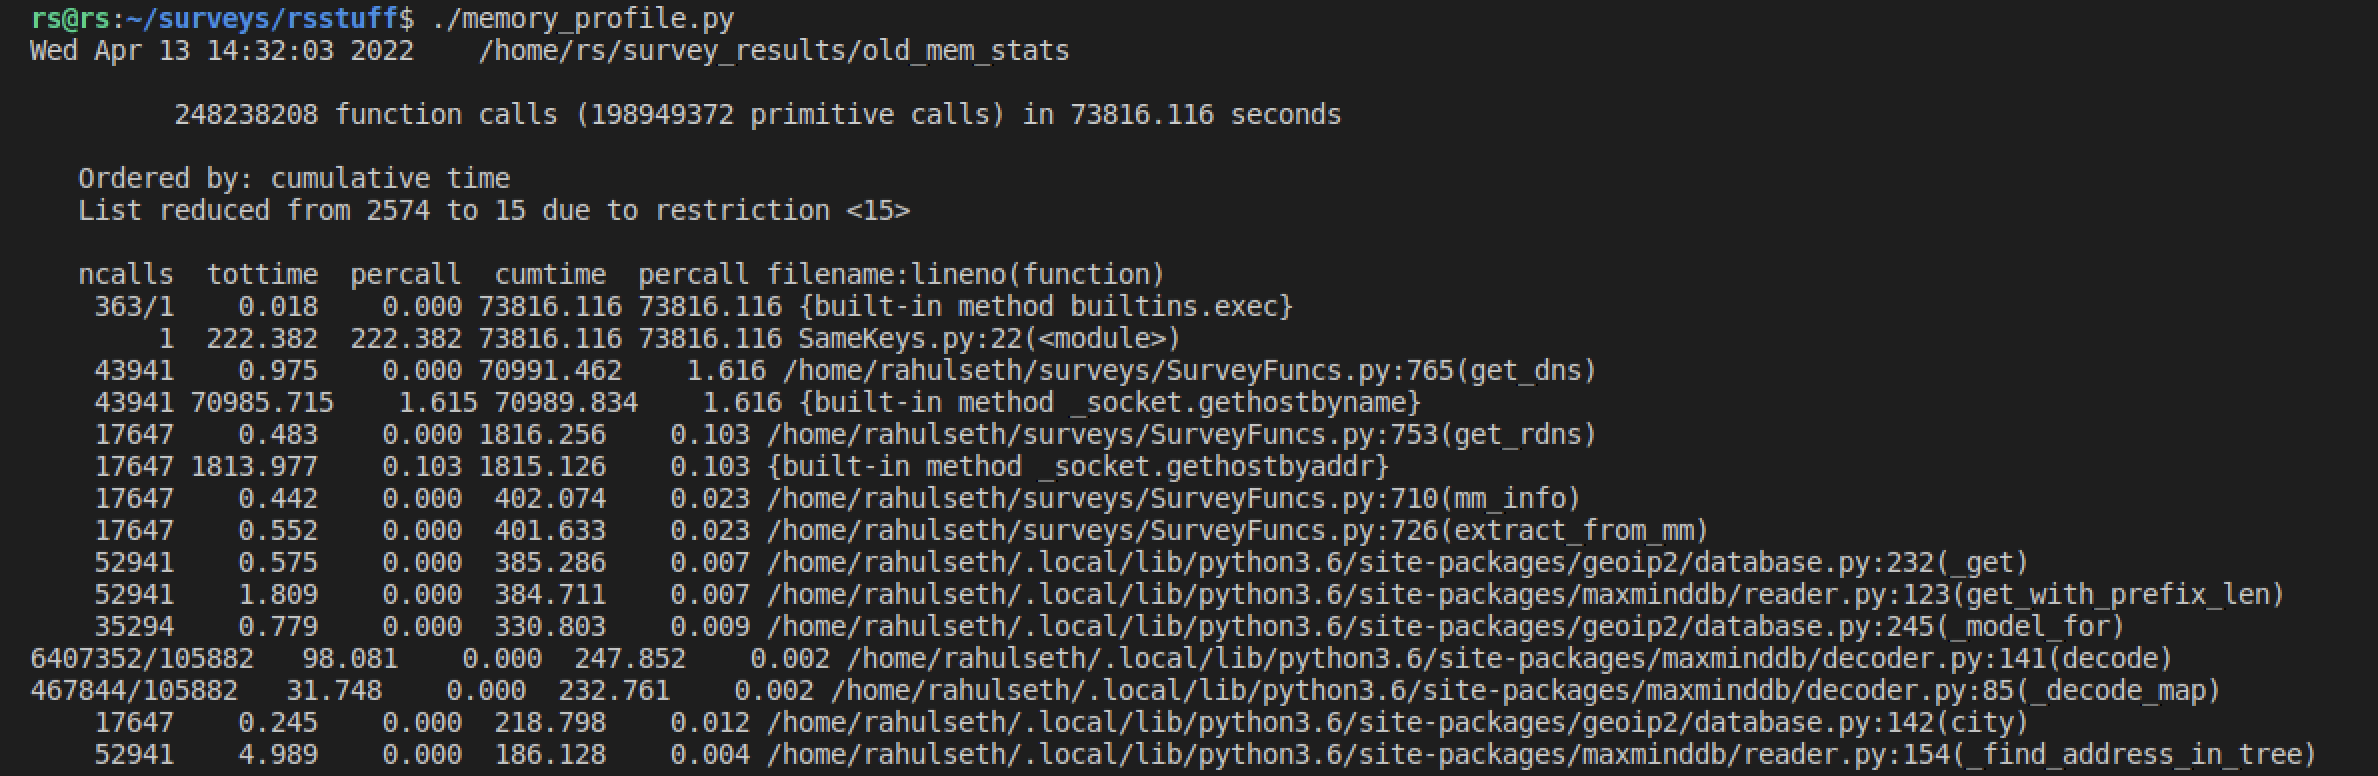
\includegraphics[width=18cm]{old_mem_profile.png}
    \caption{Memory Profile before Refactoring}
    \label{fig:oldmemprof}
\end{figure}

\noindent Figure~\ref*{fig:oldmemprof} depicts the output upon profiling the code before any optimisation or major refactoring was carried out. 
The above profiling was done on the same data that was used to carry out the data analysis. Referring to the figure, it is visible the total 
execution time of the program was about 73816 seconds, but most of the time was consumed by the function \verb|gethostbyname()| that is 
used to perform DNS lookups on the names parsed out from the metadata. The names include banner information and 
subject alternative names (SANs). Once this bottleneck was identified, alternative DNS resolution solutions were looked at 
(discussed in the section below), and different benchmark tests were created in order to see the timing of each solution and which met the 
scope of the project.

\subsection{DNS Resolving}
After memory profiling the program, it was found that the DNS resolution part of the code was consuming much time. Few alternate solutions 
were explored for faster resolution to decrease the run time. Reasons why DNS resolution was creating a bottleneck were investigated. 
Some solutions that were looked at to mitigate this problem were: DNSpython, MassDNS Resolver, Berserker Resolver, and Stubby plus Unbound. 
A benchmark timing test was created for the four, and it was found that using a combination of stubby plus unbound was the fastest among them. 
The problem with the first three options were as follows: 
\begin{itemize}
    \item MassDNS~\cite{blechsch83:online} is used to make queries in the range of millions to billions and was not fitting the scope of the project. 
    \item DNSpython~\cite{dnspytho38:online} had the same performance as \verb|gethostbyname()| function in the socket library 
    unless a timeout value was set for lookups which was not the most efficient way to solve this issue.
    \item Berserker Resolver~\cite{berserke53:online} had an upgrade in performance but used DNSpython in the backend. 
\end{itemize} 
A more permanent solution was required, and that was using a combination of two open-source tools called Unbound and Stubby. Unbound is a 
validation, recursive, caching DNS resolver that is designed to be fast and lean and provides modern services like DNS over TLS and DNS over HTTPS, 
which allows encryption while making name resolutions~\cite{NLnetLab67:online}. Stubby is an application that acts as a local DNS stub 
resolver and uses DNS-over-TLS for resolutions. The combination of Unbound and Stubby was used to speed up the DNS resolution for our program.\\ 
Unbound was used behind stubby, and all queries made using Unbound were forwarded to Stubby. Since Stubby uses DNS over TLS, which is assigned to port 853 as compared to 
traditional DNS that operates on port 53. The configuration had to be set up for the same. Before testing the code with this combination, 
Wireshark was used to analyse the traffic on port 853 while performing DNS lookups to ensure it was functioning as expected. 
Wireshark is a network packet analyser that captures in-depth detail about the captured packet~\cite{Chapter148:online}.
\newpage

\section{Challenges}
\label{challenges}
This project came across a few expected challenges. One of the significant challenges was configuring and visualising the ZMap and ZGrab tools. Although it was relatively 
easy to understand how ZMap works and how the output would look, the ZGrab posed a real challenge since the output from the tool was in JSON and involved heavy nesting.
Development for this program was done using various Linux systems, and the table below shows the Virtual Machines that were set up and 
their purpose during the course of this project.

\begin{table}[h!]
    \centering
    \begin{tabular}{|c|c|}
        \hline
        Ubuntu Version  &   Purpose\\
        \hline
        22.04   &   Development \\
        \hline
        21.04   &   Target VM for testing ZGrab\\
        \hline
        18.04   &   Testing\\
        \hline
    \end{tabular}
    \caption{VM Setup}
    \label{vm:vmsetup}

    \quad
    
    \begin{tabular}{|c|c|}
        \hline
        Service  &   Protocol\\
        \hline
        Apache Server   &   HTTPS,SSH\\
        \hline
        Dovecot   &   IMAP and POP3\\
        \hline
        Postfix   &   SMTP\\
        \hline
    \end{tabular}
    \caption{Target VM Setup}
    \label{tab:targetvmsetup}
\end{table}

\noindent The target VM was set up with different servers available in open-source that offered the protocols required. Table~\ref*{tab:targetvmsetup} 
shows the server setup on the target VM and the protocols provided by each. These servers were set up using minimal configurations to test the ZGrab 
tool over localhost. Since the program used a Python Script to use the ZGrab tool and performed IP checks according to the MaxMind databases, 
the reserved IP addresses could not be used as MaxMind does not recognise them as it operates the same blacklist as ZMap. 
Due to this, the ZGrab tool was tested manually using the command-line interface for each protocol by adding multiple IPv4 addresses and mapping 
them to each service configured.





\chapter{Results and Discussion} 
%%reuslts 
This chapter explains the results obtained after carrying out the Data Analysis process. It demonstrates key reuse across numerous hosts 
through the help of graph visualisations and other tables to provide an in-depth analysis of the clusters. This chapter also provides 
insights into the results obtained after optimisation and how it affected the program's run time and memory usage.

\section{Overview of Results}
\label{overview}
\begin{figure}[h!]
    \centering
    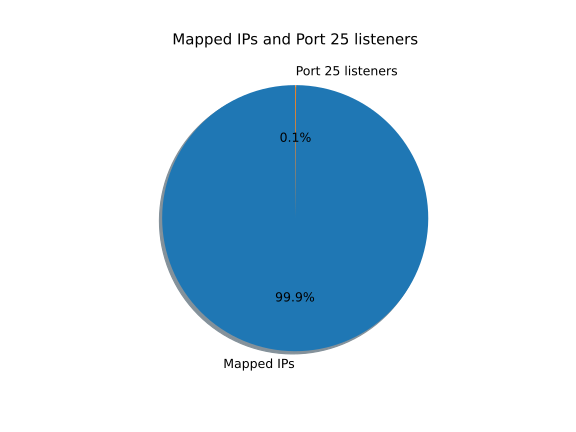
\includegraphics[width=13cm]{mapped-p25.png}
    \caption{IE Port 25 listeners}
    \label{fig:mappedp25}
\end{figure}
\pagebreak

\begin{figure}[h!]
    \centering
    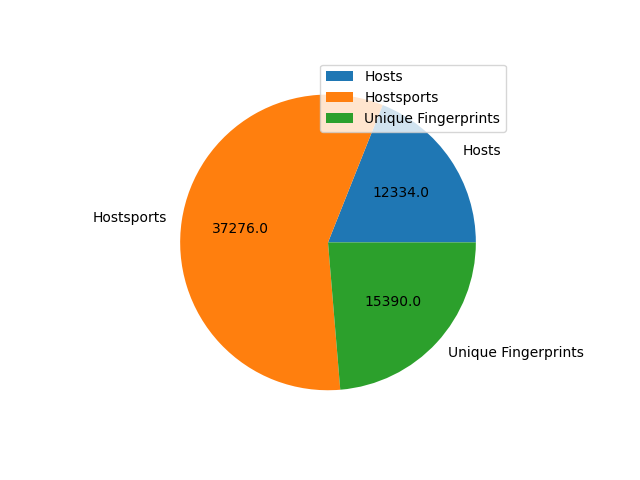
\includegraphics[width=14cm]{hostsports.png}
    \caption{Hosts v/s Host Ports v/s Fingerprints}
    \label{fig:hostports}
\end{figure}

\noindent Figure~\ref{fig:mappedp25} shows the number of IP addresses identified by ZMap as port 25 listeners. Out of the total IPs for Ireland (16421058), only 17,665 
were identified as mail servers making it 0.1\% of the total IPv4s assigned to Ireland.\\\\
12,333 hosts did some cryptography out of the 17,665 hosts identified as port 25 listeners, as indicated by figure~\ref*{fig:hostports}. 
Out of 12,333, about 37,276 host-ports combinations did some cryptography, but there were only 15,390 (41\%) unique fingerprints seen throughout the scans.
As only 41\% fingerprints were unique, it can be concluded that there is key sharing among hosts. The sections below further analyse this key 
reuse and provide analysis of some of the intriguing clusters found. 

\section{Protocol Versions}

\subsection{Cryptography per port Count}
\begin{figure}[h!]
    \centering
    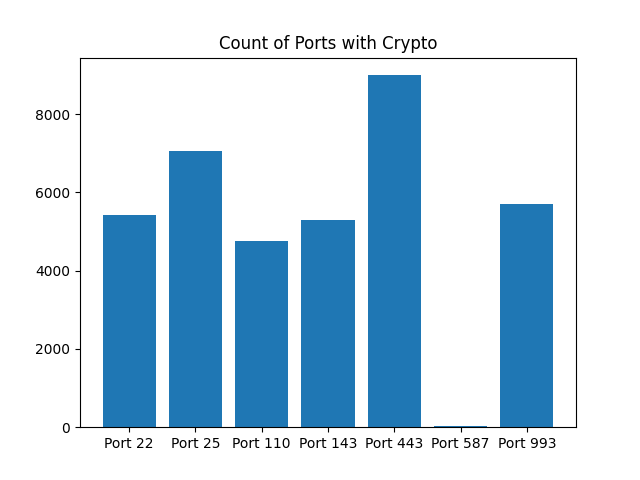
\includegraphics[width=12cm]{crypto-count.png}
    \caption{Ports that offer Crpto}
    \label{fig:cryptocount}
\end{figure}

\noindent Figure~\ref{fig:cryptocount} (below) depicts how many ports do some sort of cryptography across all IP addresses. Surprisingly, only 32 hosts on port 587 were found 
to be offering cryptographic services, and port 443 had the most number of hosts.
\subsection{SSH Versions}
\begin{figure}[h!]
    \centering
    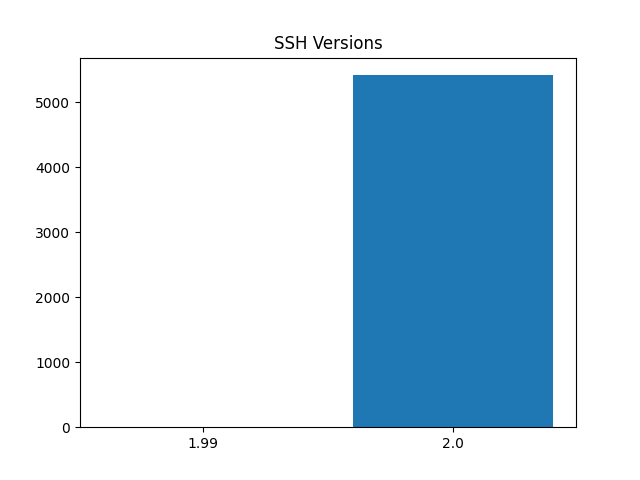
\includegraphics[width=10cm]{sshvers.png}
    \caption{SSH Versions}
    \label{fig:sshvers}
\end{figure}
\noindent Figure~\ref{fig:sshvers} above represents the SSH versions seen throughout the scans. Only two SSH versions are operating with only one host using them. 
SSH 1.9 and the rest of them using SSH 2.0. SSH 2.0 was introduced in 2006 and is the current standard version of SSH introduced by the IETF.
It provides significant improvements in terms of efficiency and security. SSH versions 1.0 and 2.0 are incompatible. Hence, SSH 1.9 was introduced by 
the IETF to provide some backward compatibility between the two versions~\cite{rfc4253}. 
\newpage

\subsection{TLS Versions}
\begin{table}[h!]
    \centering
    \begin{tabular}{|c|c|c|c|c|c|}
        \hline
        port  & SSLv3 & TLSv1.0 & TLSv1.1 & TLSv1.2 & Total  \\ \hline
        p25 & 0 & 120 & 4 & 6930 & 7054 \\ \hline
        p110 & 1 & 166 & 3 & 4600 & 4770 \\ \hline
        p143 & 0 & 179 & 3 & 5108 & 5290 \\ \hline
        p443 & 0 & 266 & 3 & 8729 & 8998 \\ \hline
        p587 & 0 & 2 & 0 & 30 & 32 \\ \hline
        p993 & 0 & 144 & 7 & 5563 & 5714 \\ \hline
        Total  & 1 & 877 & 20 & 30960 & 31858 \\ \hline
    \end{tabular}
    \caption{TLS Versions}
    \label{table:tlsvers}
\end{table}

\noindent Table~\ref*{table:tlsvers} shows the TLS versions seen throughout the scans irrespective of the IP address belonging to a cluster. Most of the TLS versions 
seen are TLS 1.2, followed by TLS 1.0, with the least SSLv3. There was no instance of TLS 1.3 in our scans. Surprisingly, it was observed 
that a significant number of hosts are still operating TLS 1.0, and some are employing TLS 1.1 even though both TLS versions have been depreciated by the 
IETF. The old versions were depreciated because of significant security flaws associated with the old versions. Some of the reasons behind 
the depreciation of TLS 1.0 and 1.1 are:
\begin{itemize}
    \item Old TLS versions require implementation using old cipher suites that are no longer desirable from a security point of view.
    \item Old versions do not support the modern and recommended cipher suites.
    \item The integrity of the handshake and the authentication process depend on SHA-1 hashes and signatures, respectively, which can easily be broken and has been superseded by SHA-2. 
\end{itemize} 
\noindent TLS 1.0 was released in 1999 and is considered to be the weakest of all TLS versions, and the IETF does explicitly not permit the use of it \cite{rfc8996}. 
This is because it is known to suffer from attacks like the BEAST due to improper implementation of the Cipher Block Chaining~\cite{rfc7457}.\\\\
Even though TLS 1.2 has also been upgraded by TLS 1.3, it was not seen during the scans. 
This might be because the TLS 1.3 upgrade is one of the most significant upgrades as compared to other TLS versions. The new upgrade introduced 
new features like 0-RTT that provide significant speed upgrades during a TLS connection establishment. Since TLS 1.3 was drastically different,
and due to middleboxes all over the internet, the TLS handshake might seem like a TLS 1.2 connection even though it is TLS 1.3~\cite{rfc8446}. 

\section{Key Reuse Results}
Five thousand eight hundred nine collisions were found, producing about 1049 clusters. The graphs below are a few of the selected clusters from 
the results. Some were selected based on the number of hosts, while others were chosen randomly.

\subsection{Cluster 15}
\begin{figure}[h!]
    \centering
    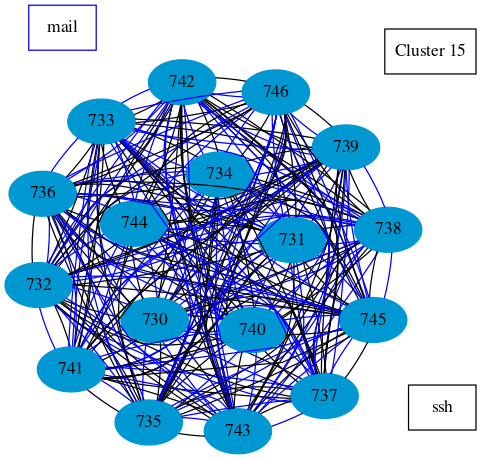
\includegraphics[width=10cm]{graph15.dot.png}
    \caption{Cluster 15}
    \label{fig:cluster15}
\end{figure}
\noindent Figure~\ref*{fig:cluster15} is the biggest pure SSH cluster and has about 15 hosts in total belonging to the same AS. There are
68 hostport combinations, with 34 of them being SSH and the other 34 being TLS ports. For both SSH and TLS,  only see one key was  
used among all hosts for both protocols.\\\\
\noindent Although Cluster 5 is the biggest SSH cluster found in our results but was not rendered due to a lack of memory in the machine. 
It has 226 hosts belonging to the same AS with about 1322 host port combinations. Out of the total host port combinations, 418 are SSH ports, 
with only one SSH key being shared. The rest of the 904 host-ports combinations are TLS ports, and one TLS key is shared among them.
\pagebreak

\subsection{Cluster 43}
\begin{figure}[h!]
    \centering
    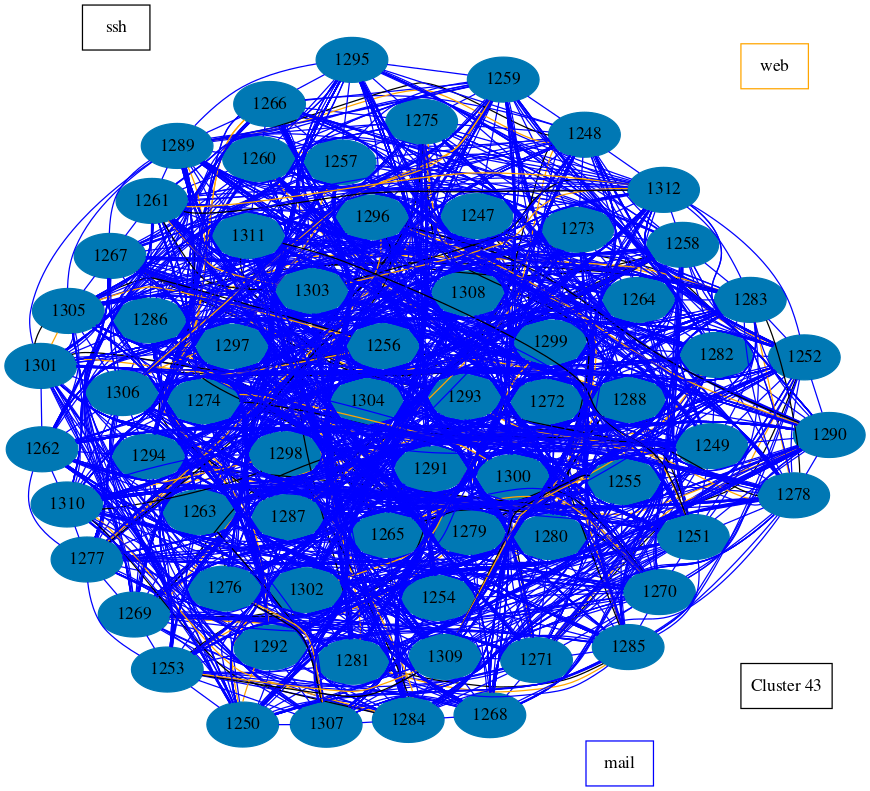
\includegraphics[width=14cm]{graph43.png}
    \caption{Cluster 43}
    \label{fig:cluster43}
\end{figure}

\noindent Figure~\ref{fig:cluster43} represents Cluster 43 from the results. It is a cluster consisting of 66 hosts sharing the same keys for SMTP, SSH and HTTPS protocols. 
All of the hosts belong to the same Autonomous System in this case. There are about 722 host-port combinations, with 86 of them being SSH. There were only 14 unique SSH keys seen for the 86 host-port combinations. Out of the 722 host-port combinations, 636 
were TLS ports with only 22 unique TLS keys seen. The AS in question here is a web-hosting service with a local presence. 
\pagebreak

\subsection{Cluster 72}
\begin{figure}[h!]
    \centering
    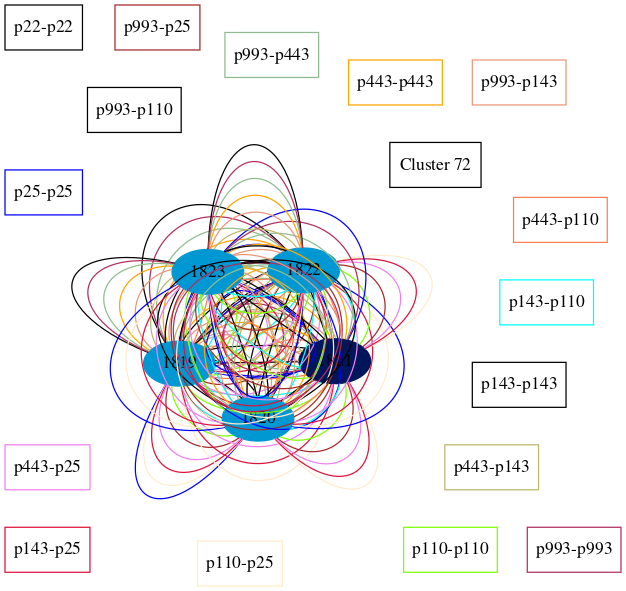
\includegraphics[width=14cm]{graph72.png}
    \caption{Cluster 72}
    \label{fig:cluster72}
\end{figure}

\noindent Figure~\ref{fig:cluster72} is an interesting one. Key sharing across almost every pair port combination is observed. There are five hosts in this cluster, 
out of which four belong to the same AS. There is key sharing across all mail protocols, but even cross-protocol key sharing among hosts for HTTPS and SMTP, IMAP and POP3 is observed. 
Upon inspection of the cluster data, it was found that the four ASes that are the same are again a web-hosting service, while the other AS seems to belong to a Telecommunications company.  
\pagebreak

\subsection{Cluster 133}
\begin{figure}[h!]
    \centering
    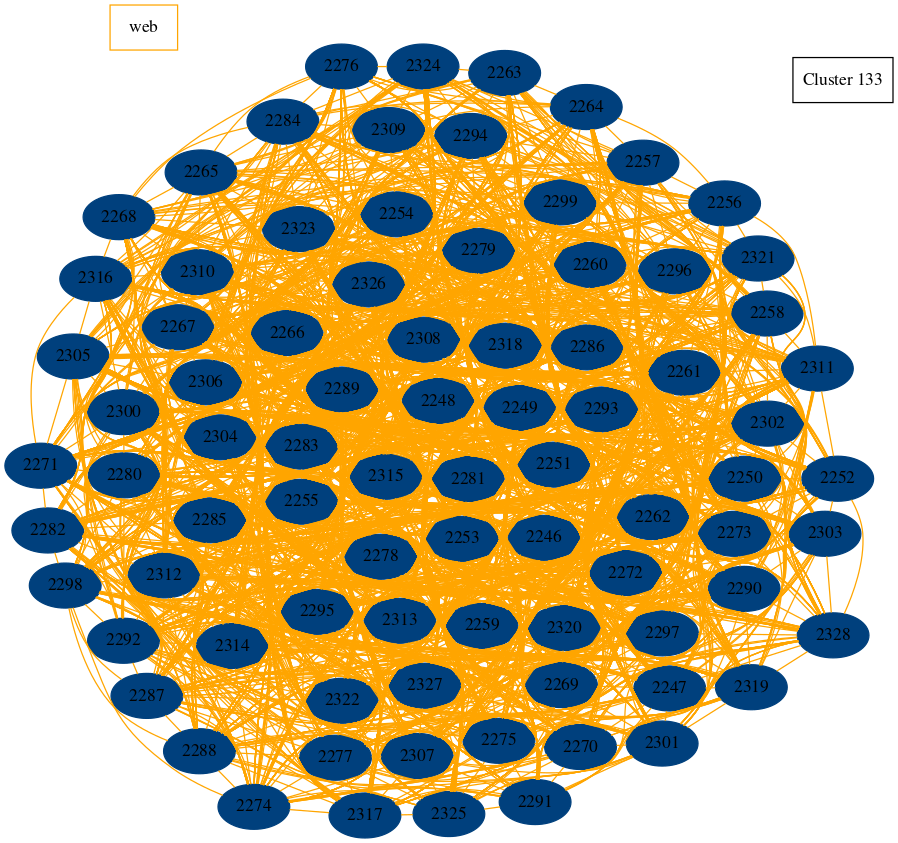
\includegraphics[width=14cm]{graph133.png}
    \caption{Cluster 133}
    \label{fig:cluster133}
\end{figure}

\noindent Figure \ref*{fig:cluster133} represents Cluster 133 from the results, and it consists of 83 hosts sharing web server keys (HTTPS). This is one of the busier clusters found in the results, and there are a few clusters 
larger than this. All 83 hosts belong to the same AS, a global web hosting service, and share keys for only port 443. There are about 166 host-port combinations, sharing only a single TLS key. 
\pagebreak

\subsection{Cluster 148}
\begin{figure}[h!]
    \centering
    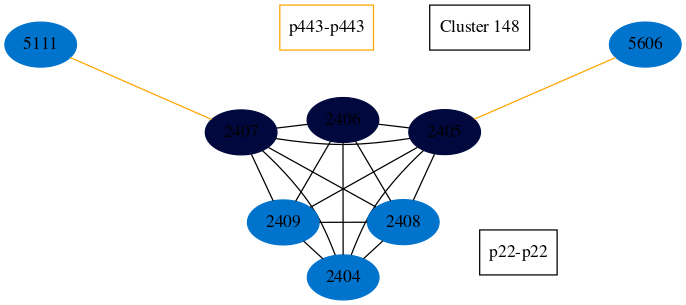
\includegraphics[width=16cm]{graph148.png}
    \caption{Cluster 148}
    \label{fig:cluster148}
\end{figure}

\noindent Figure \ref{fig:cluster148} represents Cluster 148 and consists of eight hosts belonging to two different ASes. Out of the eight, three belong to the same AS and 5 to a different one.  
All hosts in the middle share keys for SSH, while the the two host \textit{5111} and \textit{5606} (refer figure) at the edges share keys 
with the hosts \textit{2607} and \textit{2605} for port 433 respectively. There are about 22 host-port combinations seen,
out of which 12 are classified as SSH, and the remaining 10 are TLS. Only 1 SSH key is shared among the 12 host-port combinations, while 3 TLS keys are shared for ten host-port combinations. The AS with three hosts belong to a local ISP, and the other one with five hosts 
belongs to a telecommunications entity with a huge local presence. 
\pagebreak

\subsection{Cluster 536}
\begin{figure}[h!]
    \centering
    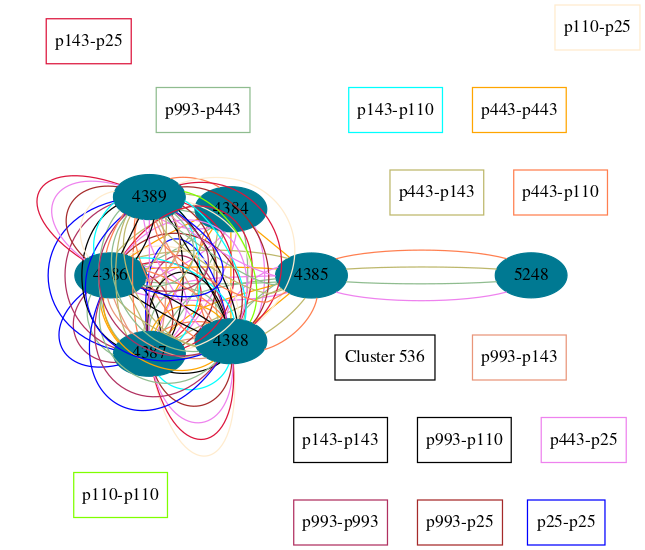
\includegraphics[width=16cm]{graph536.png}
    \caption{Graph 536}
    \label{fig:cluster536}
\end{figure}
\noindent Figure~\ref{fig:cluster536} represents Cluster 536 and has about seven hosts, all belonging to the same AS. There are seven hosts with 58 
hosts-port combinations and only four unique TLS keys. Key reuse across almost port combinations is seen here. The max key usage for a single seen 
was 38 times in this cluster. The hosts involved in this cluster seem to provide web services like mail and DNS using cloud platforms.
\pagebreak

\subsection{Cluster 786}
\begin{figure}[h!]
    \centering
    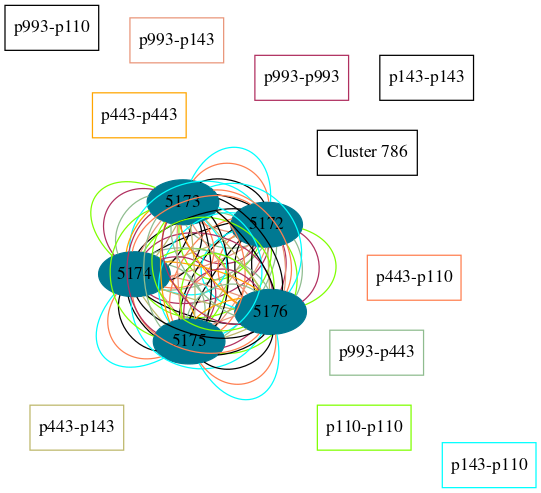
\includegraphics[width=12cm]{graph786.dot.png}
    \caption{Cluster 786}
    \label{fig:cluster786}
\end{figure}
\noindent Figure~\ref*{fig:cluster786} consists of five hosts; all belong to the same AS and share keys for TLS. There were 40 host-port combinations 
with only two TLS keys, out of which one of the keys was reused 38 times. This cluster is interesting as one of the hosts has a domain name that belongs to 
Trinity College, Dublin. The domain name associated was on port 443 (HTTPS). For instance, if Trinity's website is ``www.tcd.ie'', the 
domain name in question here looked like ``www.tcdxxxx.ie''. The AS here is a telecommunications company in Ireland. 
\pagebreak

\subsection{TLS Cipher Suites}
The TLS Cipher Suites seen for the selected clusters:
\begin{figure}[h!]
    \centering
    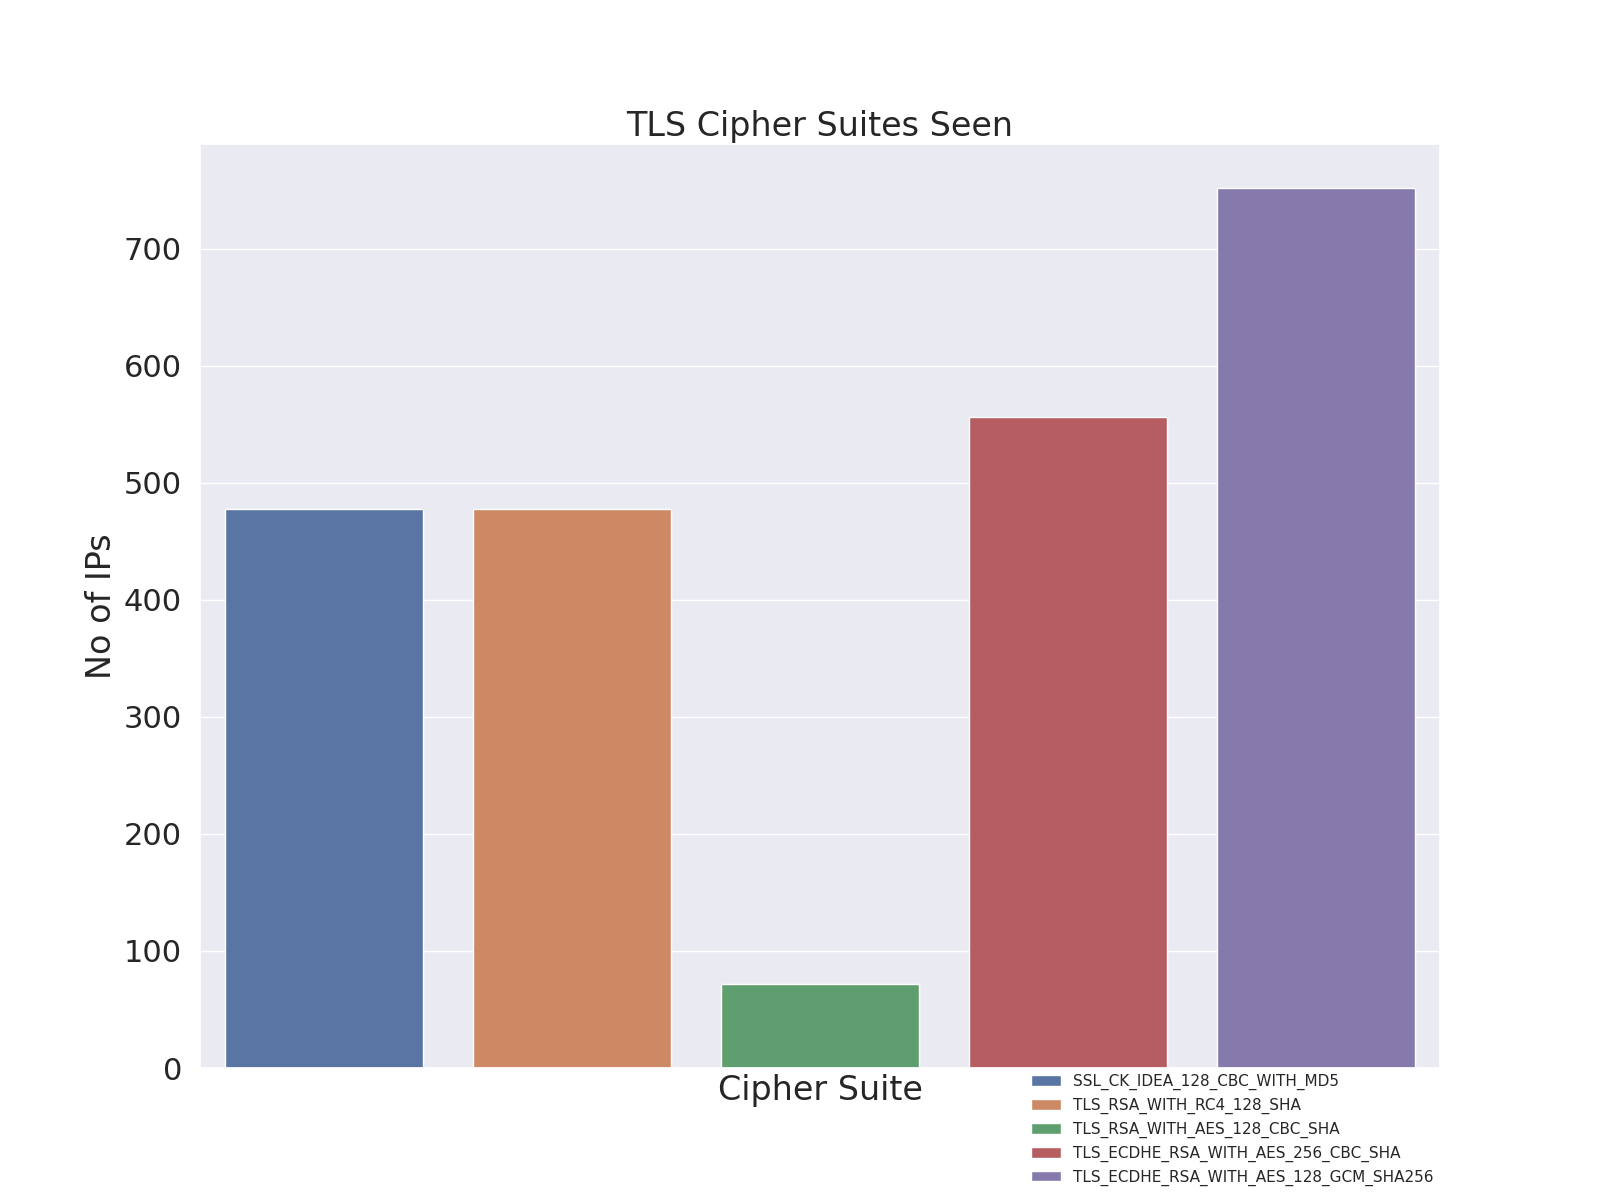
\includegraphics[width=17cm]{newgraph.png}
    \caption{TLS Cipher Suites}
    \label{fig:tlsciphers}
\end{figure}

\noindent Table~\ref*{fig:tlsciphers} shows the TLS cipher suites seen for the selected clusters. The most common cipher suite was found to be \verb|TLS_ECDHE_RSA_WITH_AES_128_GCM_SHA256| followed by 
\verb|TLS_ECDHE_RSA_WITH_AES_256_CBC_SHA|. Many hosts were using \verb|TLS_RSA_WITH_RC4_128_SHA|, which is known to have cryptographic weaknesses. The IETF prohibits the 
use of any RC4-based Cipher Suite as they do not provide desired security~\cite{rfc7465}. The least used Cipher Suite was \verb|TLS_RSA_WITH_AES_128_CBC_SHA|.
There were also significant hosts using the \verb|SSL_CK_IDEA_128_CBC_WITH_MD5| cipher that was introduced in 1992. Since then extensive studies have 
been carried out on it and is known to be broken.~\cite{rfc6151}
\newpage

\section{Post Refactoring and Optimisation}
This section discusses the results obtained after code refactoring. The profiling is done again after 
making the changes and modifications in the program. There is also a timing graph presented 
that compares the average time per IP spent analysing using the two DNS setups.
\begin{figure}[!h]
    \centering
    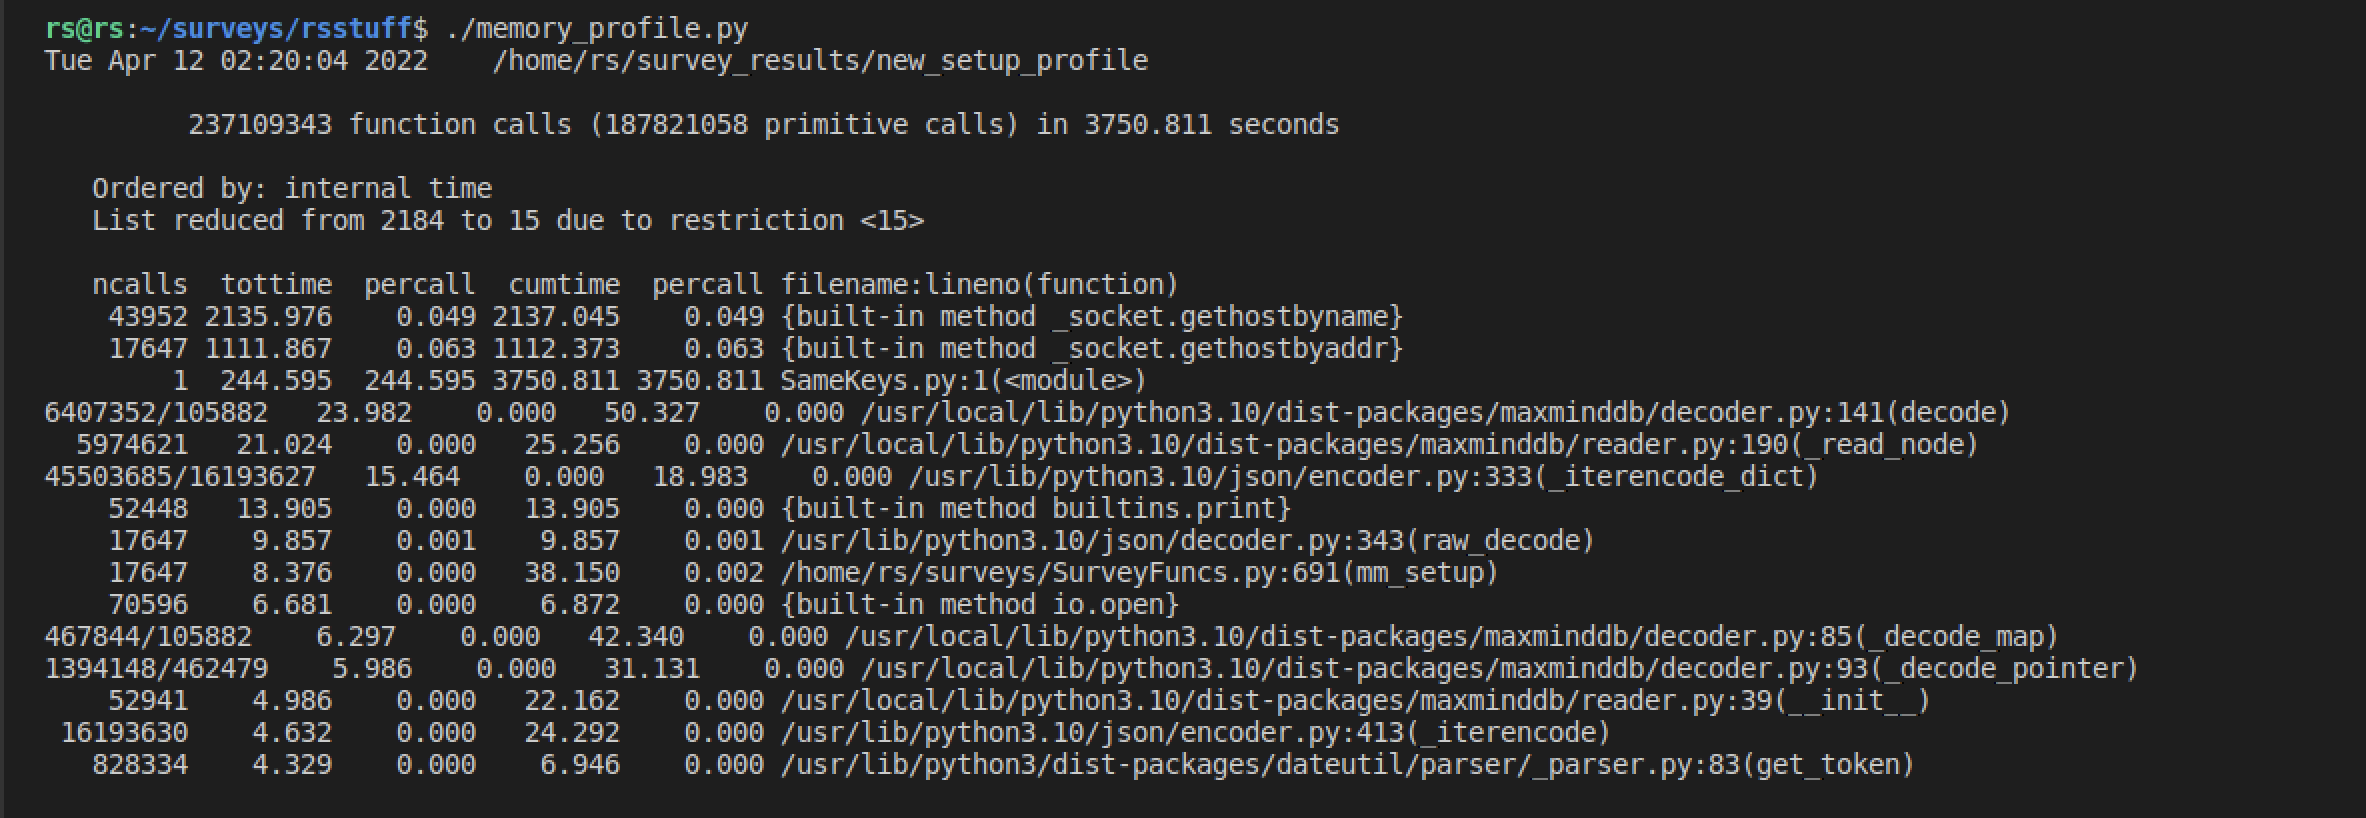
\includegraphics[width=17cm]{new_mem_profile.png}
    \caption{Memory Profile after Refactoring}
    \label{fig:memprofileafter}
\end{figure}

\noindent Figure~\ref*{fig:memprofileafter} represents the memory profiling after refactoring and optimisation as depicted in the sections above. 
The runtime for data processing and analysis was reduced from 73816 seconds to 3750 seconds. In addition, after refactoring, the number of recursive calls 
were reduced, contributing to optimising the memory consumption as recursive methods can take up a lot of memory. The new DNS setup 
significantly improved the runtime of the program, and this might be due to the following factors:
\begin{itemize}
    \item Typical DNS setups rely on servers supplied by ISPs that might be slow. 
    \item Configurations for caching might not be adequately implemented by the ISP, which may contribute to slow lookups.~\cite{HowandWh90:online}
\end{itemize}
\pagebreak

\begin{figure}[h!]
    \centering
    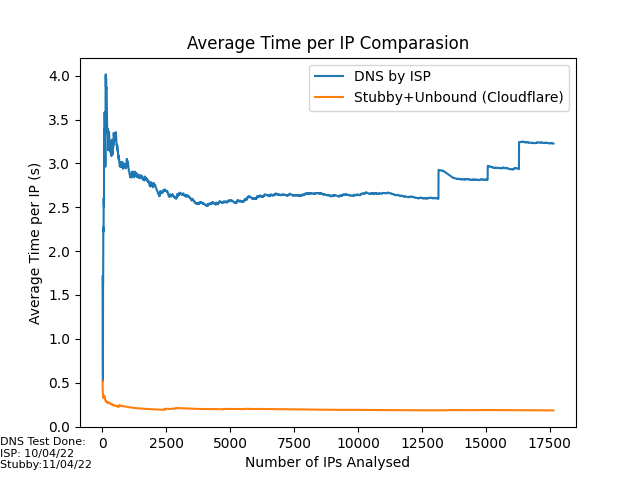
\includegraphics[width=15cm]{newdnscomp.png}
    \caption{DNS Setup Comparisons}
    \label{fig:dnscomps}
\end{figure}

\noindent Figure~\ref*{fig:dnscomps} above shows the difference between the average time spent per IP when using the two DNS setups.
The average time processing each IP was bought down to 0.15s from 3.4s when using the default setup. This might be due to the following 
reasons:

\begin{itemize}
    \item Using Unbound, one can get more control over their DNS setup as it allows one to configure the DNS servers one might want to use. 
    \item It will also cache all queries made for faster lookups the next time. 
    \item Using Stubby allows one to use DNS over TLS for sending queries to resolvers. It allows for increased privacy. 
    \item Since Unbound is not as advanced as Stubby and does not have the provision to use the same TLS connection for queries, a combination
    of the two can help speed things up. Stubby can use the same TLS connection to make multiple queries, saving the overhead and time to open up 
    a new connection for each query.~\cite{NLnetLab67:online, DNSPriva7:online}
\end{itemize}

\chapter{Conclusions and Future Work}
%%conclusions 
\section{Conclusions}
Both research and personal objectives were outlined in section 1.2 to guide the project and provide a means 
to complete the project in the time frame given. This chapter discusses the goals completed and provides conclusions on the work carried out.

\subsection{Goals Revisted}
One of the primary goals of this project was to migrate the code for the current surveying tool to Python3 and refactor it along the way 
to optimise it. The refactoring and migration process was carried out successfully, and there were significant improvements in the program 
by making use of new functionalities available in Python3. Since support for Python2 has depreciated, even though some may argue the benefits 
of Python2 over Python3 but since there is an industry-wide shift towards the adaptation of Python3, this would prove beneficial if other 
entities wish to use this program. In addition, the migration makes it more accessible and easy to run. While carrying out the refactoring process, 
the Python Enhancement Proposal 8 (PEP8)~\cite{pep8} was followed to standardise the code to industry standards to increase understanding of the program. 
Following this convention allowed to maintain a single coding style throughout the program amongst many scripts, which could benefit other entities later if 
they wish to make changes to the program to fit their needs. All technologies used for this project, like Maxmind, ZMap and ZGrab, were upgraded to their latest versions.\\\\
The program's methodologies and design should allow other entities or institutions to carry out scans for different populations. They can replicate the same work as carried out here with ease. 
The program was updated to scan populations using data from the Maxmind database, and it also has provisions to do so with the Censys databases. 
Although it was not possible to upgrade the program to work with the updated versions of the Censys metadata due to Censys going commercial, 
attempts were made by contacting them to get some sample data to extend this work. However, unfortunately, Censys did not provide the data needed to upgrade this program.\\\\
Another goal of this project was to add port 853 (DNS over TLS) to the scans parameters. Code had to be written in Golang, and 
integration tests had to be run using the ZGrab integration tools available. However, it was unsuccessful due to a lack of programming experience 
in Golang and time constraints. Although a simple banner grab over port 853 using TLS was successfully added, it was not the most efficient 
way to go about it. 

\subsection{Final Remarks}
Overall, all goals but adding port 853 were accomplished, and there is still widespread key reuse seen, as proven back in 2018 by Dr.~Farrell. 
However, key reuse between SSH and other protocols that use TLS was not seen as was the same case in 2018~\cite{cryptoeprint:2018:299}. 

\newpage
\section{Future Work}
This section discusses some of the possible extensions of this work. 

\subsection{Scanning other Countries and IPv6 address Space}
Due to the time constraints, only a couple of scans for Ireland were able to be carried out, and data analysis was only done on one of the scans. Still, one could get a better understanding of some of the causes behind this key reuse by carrying out scans over a long period at regular 
intervals. While the accuracy of these scans is acceptable for this project, one could extend this work to distinguish between hosts that 
operate with more than one IPv4 address, i.e.~multi-homed hosts. Currently, the program can not differentiate between multi-homed and 
single-homed hosts. Still, introducing some techniques to distinguish between the two would provide a more accurate picture of the key 
reuse scenario for a population. Another possible extension of this work would be to scan the IPv6 addresses space.

\subsection{Adding Additional Protocols}
An exciting extension would be to add additional protocols to scan for, like the MQ Telemetry Transport Protocol (MQTT) used by IoT devices and 
adopted widely. MQTT has provisions for using TLS, and since the number of IoT devices is growing exponentially, they have a reputation for
being insecure. It would be interesting to see if there is key reuse across these protocols.  

\subsection{Database Management}
A place where this work could be improved upon is by improving data management. Since a large amount of data is captured using JSON and each 
structure is highly sparse, one could look at integrating databases like Elasticsearch, which is an open-source NoSQL database that can
be used to store unstructured data and query it with ease using SQL commands~\cite{FreeandO95:online}. This could be highly beneficial 
for entities carrying out scans for a considerable period, gathering a lot of metadata.  









\addcontentsline{toc}{chapter}{Bibliography} 
\bibliographystyle{apalike}
\bibliography{refs}
\addcontentsline{toc}{chapter}{Appendix} 
\appendix
\chapter{Sample Scan Data}
\begin{lstlisting}
    s{
  "ip": "XX.XX.XX.XX",
  "writer": "FreshGrab.py",
  "p22": {
    "ip": "XX.XX.XX.XX",
    "data": {
      "ssh": {
        "status": "connection-timeout",
        "protocol": "ssh",
        "result": {},
        "timestamp": "2022-04-02T01:40:09Z",
        "error": "dial tcp XX.XX.XX.XX:22: connect: connection refused"
      }
    }
  },
  "duration": 0.5397200584411621,
  "average": 4.158559069103385,
  "p25": {
    "ip": "XX.XX.XX.XX",
    "data": {
      "smtp": {
        "status": "application-error",
        "protocol": "smtp",
        "result": {
          "banner": "XXXXX\r\n",
          "starttls": "454 4.3.3 TLS not available after start\r\n"
        },
        "timestamp": "2022-04-02T01:40:09Z",
        "error": "SMTP error code 454 returned from STARTTLS command (454 4.3.3 TLS not available after start)"
      }
    }
  },
  "p110": {
    "ip": "XX.XX.XX.XX",
    "data": {
      "pop3": {
        "status": "connection-timeout",
        "protocol": "pop3",
        "timestamp": "2022-04-02T01:40:09Z",
        "error": "dial tcp XX.XX.XX.XX:110: connect: no route to host"
      }
    }
  },
  "p143": {
    "ip": "XX.XX.XX.XX",
    "data": {
      "imap": {
        "status": "connection-timeout",
        "protocol": "imap",
        "timestamp": "2022-04-02T01:40:09Z",
        "error": "dial tcp XX.XX.XX.XX:143: connect: no route to host"
      }
    }
  },
  "p443": {
    "ip": "XX.XX.XX.XX",
    "data": {
      "http": {
        "status": "success",
        "protocol": "http",
        "result": {
          "response": {
          }
          }
            }
          }
        },
        "timestamp": "2022-04-02T01:40:09Z"
      }
  },
  "p587": {
    "ip": "XX.XX.XX.XX",
    "data": {
      "smtp": {
        "status": "connection-timeout",
        "protocol": "smtp",
        "timestamp": "2022-04-02T01:40:10Z",
        "error": "dial tcp XX.XX.XX.XX:587: connect: no route to host"
      }
    }
  },
  "p993": {
    "ip": "XX.XX.XX.XX",
    "data": {
      "imap": {
        "status": "connection-timeout",
        "protocol": "imap",
        "timestamp": "2022-04-02T01:40:10Z",
        "error": "dial tcp XX.XX.XX.XX:993: connect: no route to host"
      }
    }
  }
}
\end{lstlisting}
\end{document}
